\chapter{Plate Model: Thickness Variation and Arbitrary Strain Fields}

The studies were also carried to estimate and cross check the variation of displacement with thickness for various types and models which are presented in this chapter. In addition, deformation in the model for an arbitrary strain field simulated by increasing the natural length of springs selectively is shown and their qualitative justifications are provided in this chapter.

\section{Thickness Variation Study}
 These studies were carried out on the model and types described in previous chapter for a loading of 2 kN applied at the centre of a suare plate simply supported along all the four edges. All the studies are for Constant Stiffness case and are presented along with the analytical prediction from Classical Plate Theory and First-order Shear Deformation theory.
 
 \subsection{Model 1}
 The result from model 1 are presented in the fig~\ref{fig:M1_t_plt} and fig~\ref{fig:M1_t_energy}. As it can be seen from the plots, as the thickness of the model increases, there are only minor variations in the deflection at centre predicted by the model for all three types and following this, there is also not much variation in the plot for energy indicating that springs contribute negligibly to the energy and most of it comes from the work done by externally applied load. This suggests that the impact of the loading on vertical deflection do not diminish with thickness and the system behaves as if it is just made of single layer. 
 
  \subsection{Model 2}
 Fig~\ref{fig:M2_t_plt} and fig~\ref{fig:M2_t_energy} show the outputs obtained using Model 2. As evident from the figures, Model 2 types predict even lesser effect of increasing thickness on vertical deflection at centre for a given concentrated load and hence indicates that increasing number of spring in the horizontal layers has an effect of diminishing the consequences of increased thickness of the model. Some of the conclusions drawn in discussion for Model 1 corrsponding to absence of variation in the plots hold here as well.
 
  \subsection{Model 3}
 The result from model 3 are shown in the fig~\ref{fig:M3_t_plt} and fig~\ref{fig:M3_t_energy}. Although the results deviate at very small thicknesses, there is very good agreement between the model prediction and analytical results. As expected, increasing the stiffness diminishes the vertical deflection at centre for the given concentrated load and as a consequence, due to smaller deflection, there is less stretching and of springs and work done by force is smaller and hence the change in energy of the systems diminish. Also, following the analytical results, deflections reach a plateau at high thicknesses and energy profiles follow accordingly.
 
 \begin{figure}[!htbp]
     \centering
     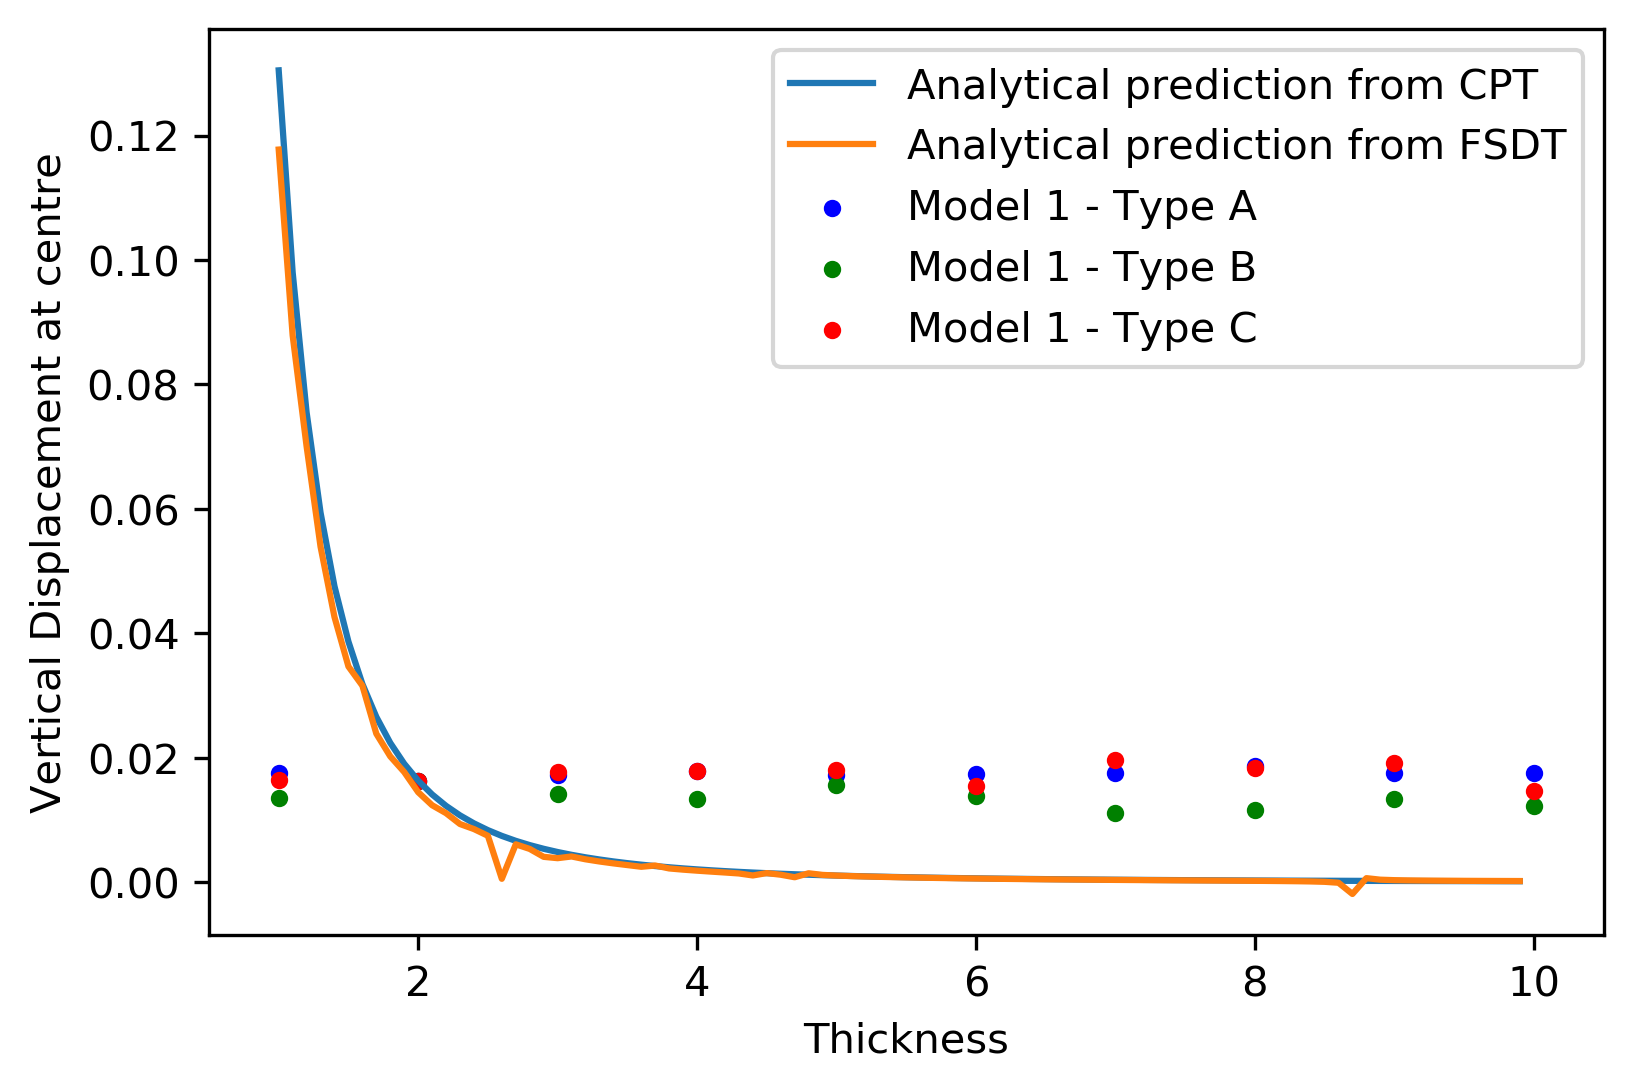
\includegraphics{Figures/M1_t_plt.png}
     \caption{Model 1 - Vertical Displacement with respect to Thickness for a Constant Vertical Load of 2 kN}
     \label{fig:M1_t_plt}
 \end{figure}
 
 \begin{figure}[!htbp]
     \centering
     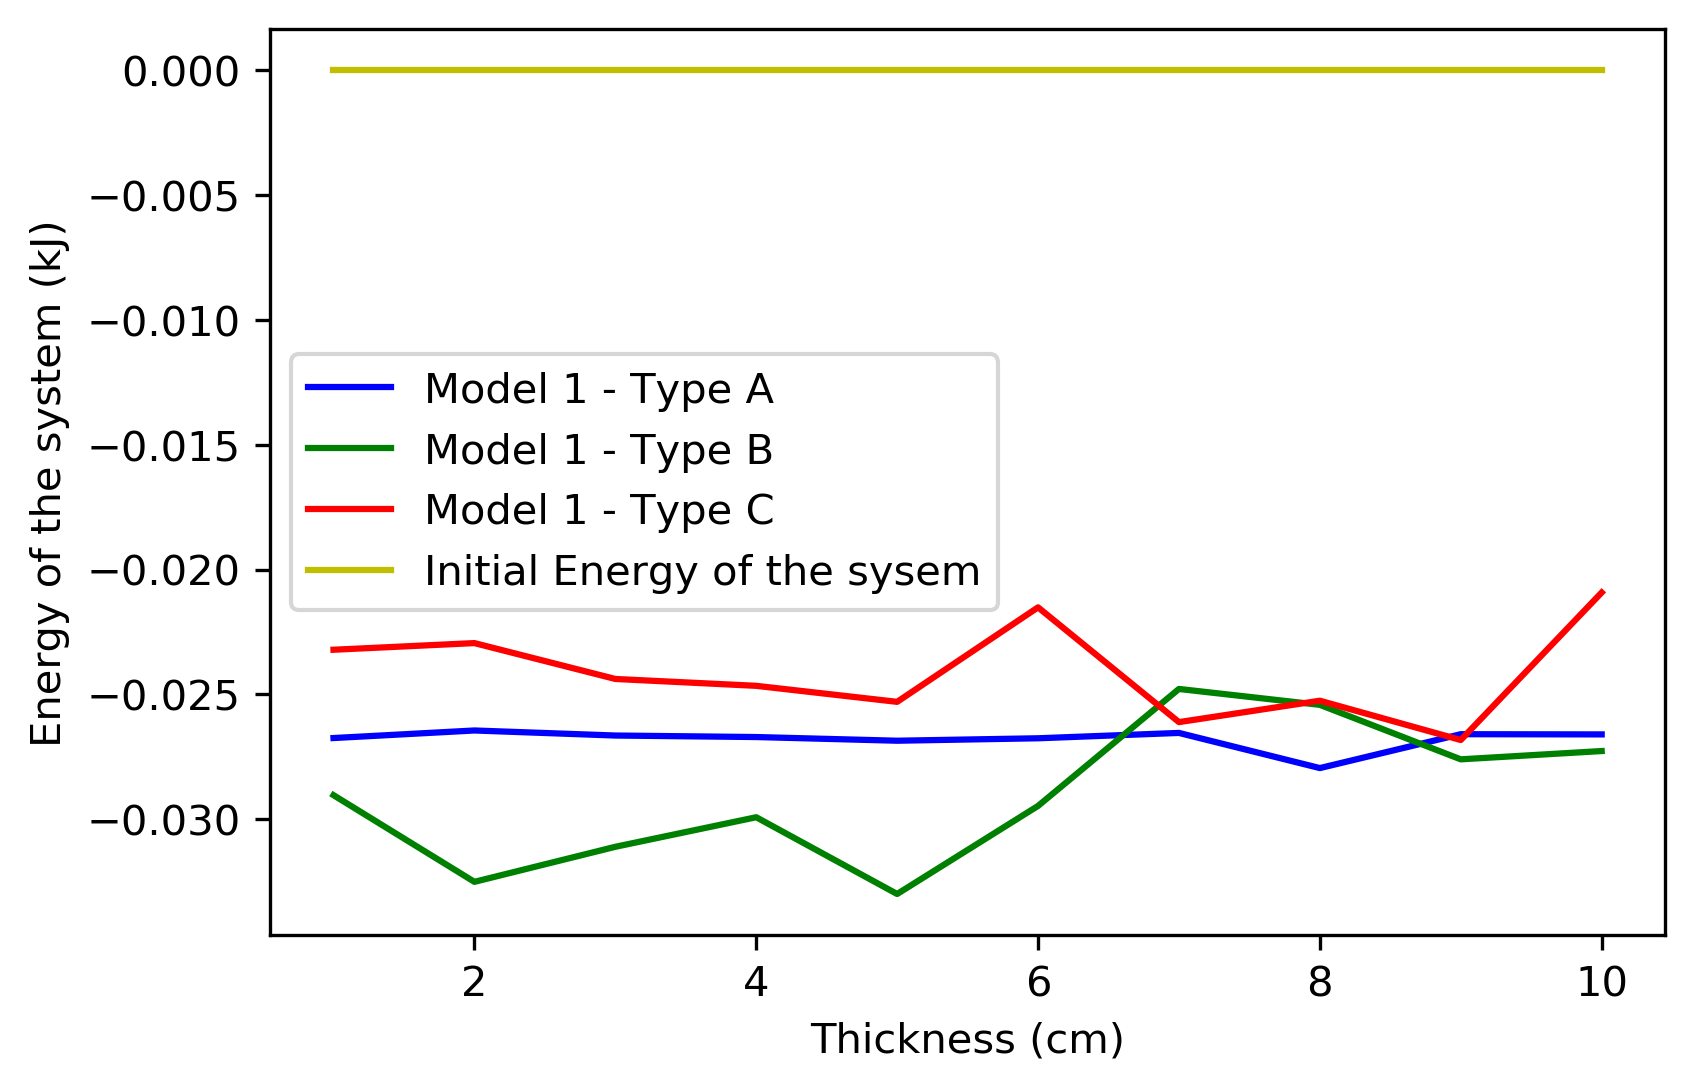
\includegraphics{Figures/M1_t_energy.png}
     \caption{Model 1 - Change in energy with respect to Thickness for a Constant Vertical Load of 2 kN}
     \label{fig:M1_t_energy}
 \end{figure}
 
 
 \begin{figure}[!htbp]
     \centering
     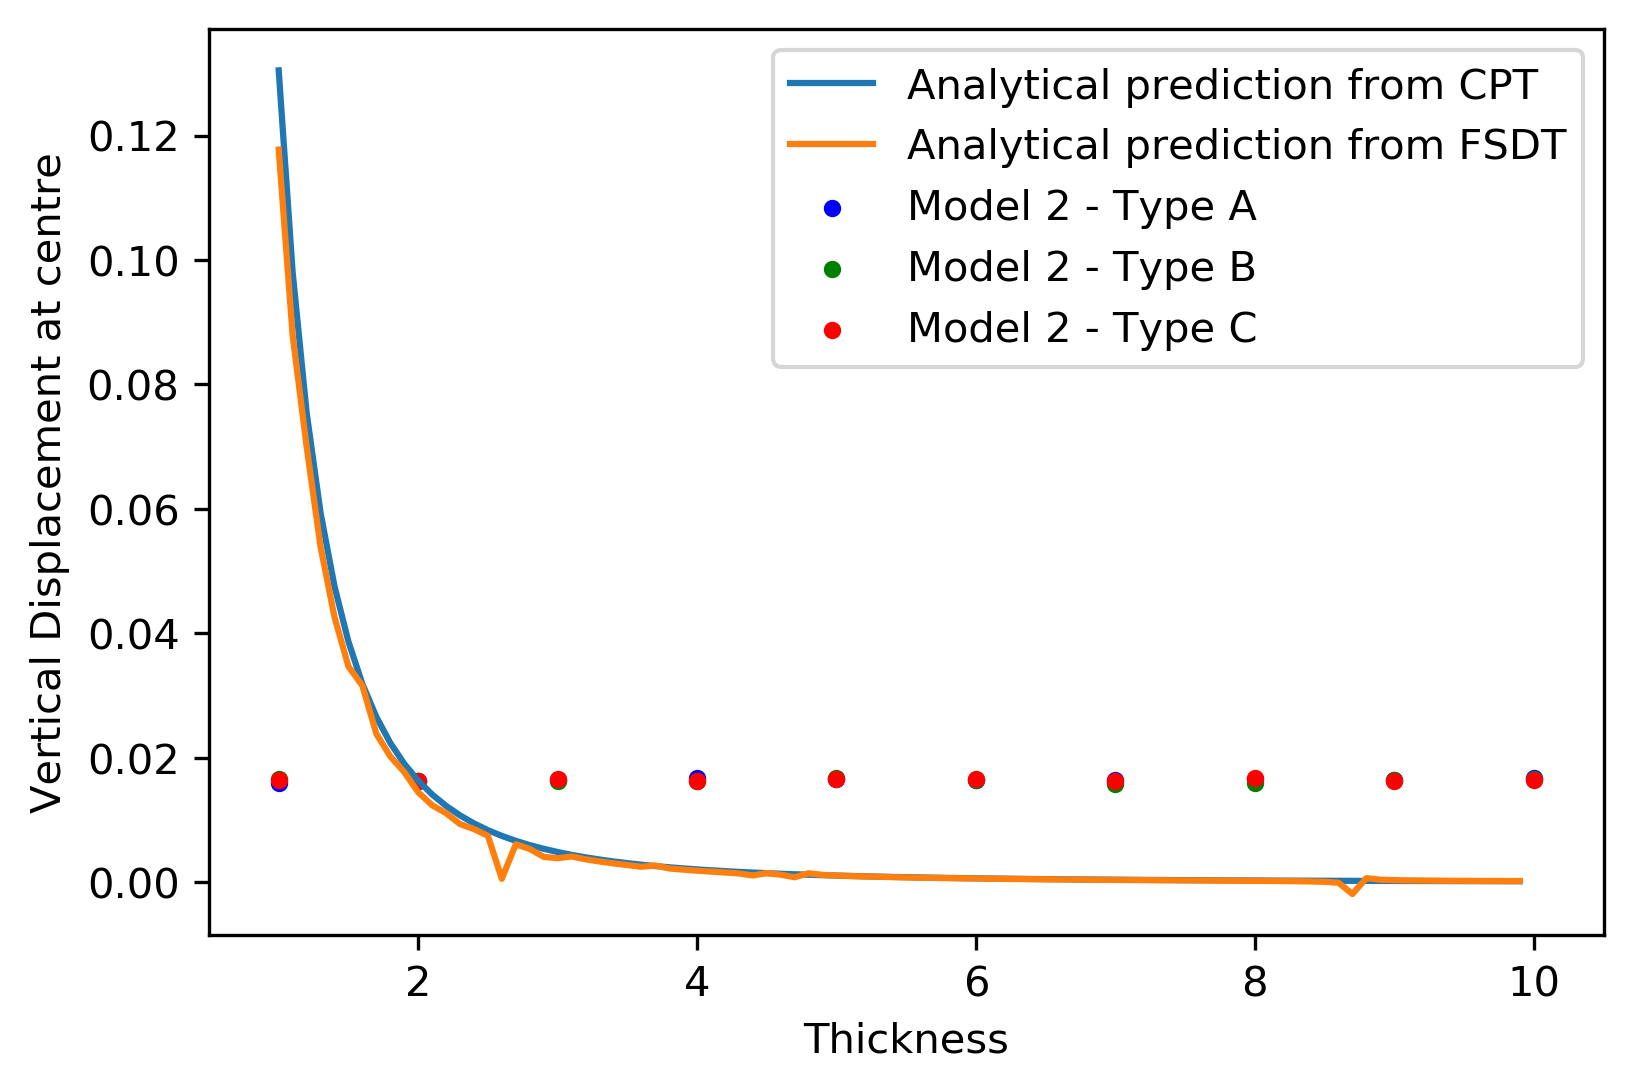
\includegraphics{Figures/M2_t_plt.png}
     \caption{Model 2 - Vertical Displacement with respect to Thickness for a Constant Vertical Load of 2 kN}
     \label{fig:M2_t_plt}
 \end{figure}
 
 \begin{figure}[!htbp]
     \centering
     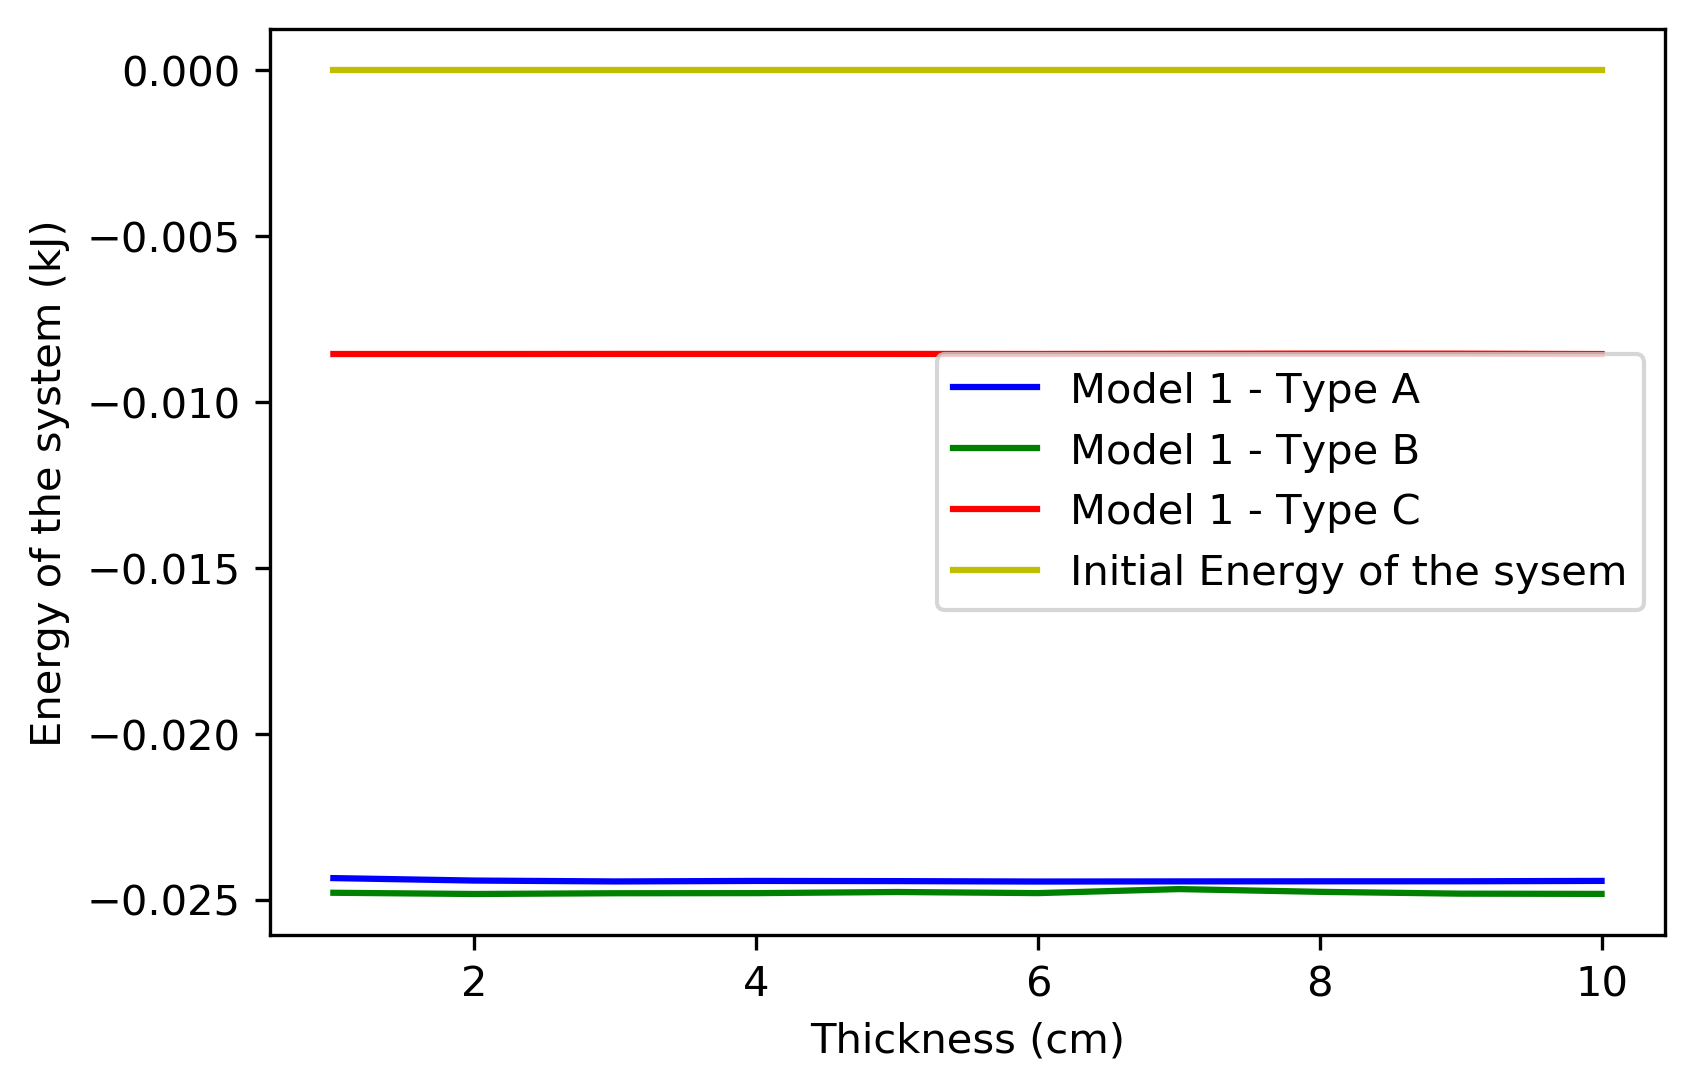
\includegraphics{Figures/M2_t_energy.png}
     \caption{Model 2 - Change in energy with respect to Thickness for a Constant Vertical Load of 2 kN}
     \label{fig:M2_t_energy}
 \end{figure}
 
 \begin{figure}[!htbp]
     \centering
     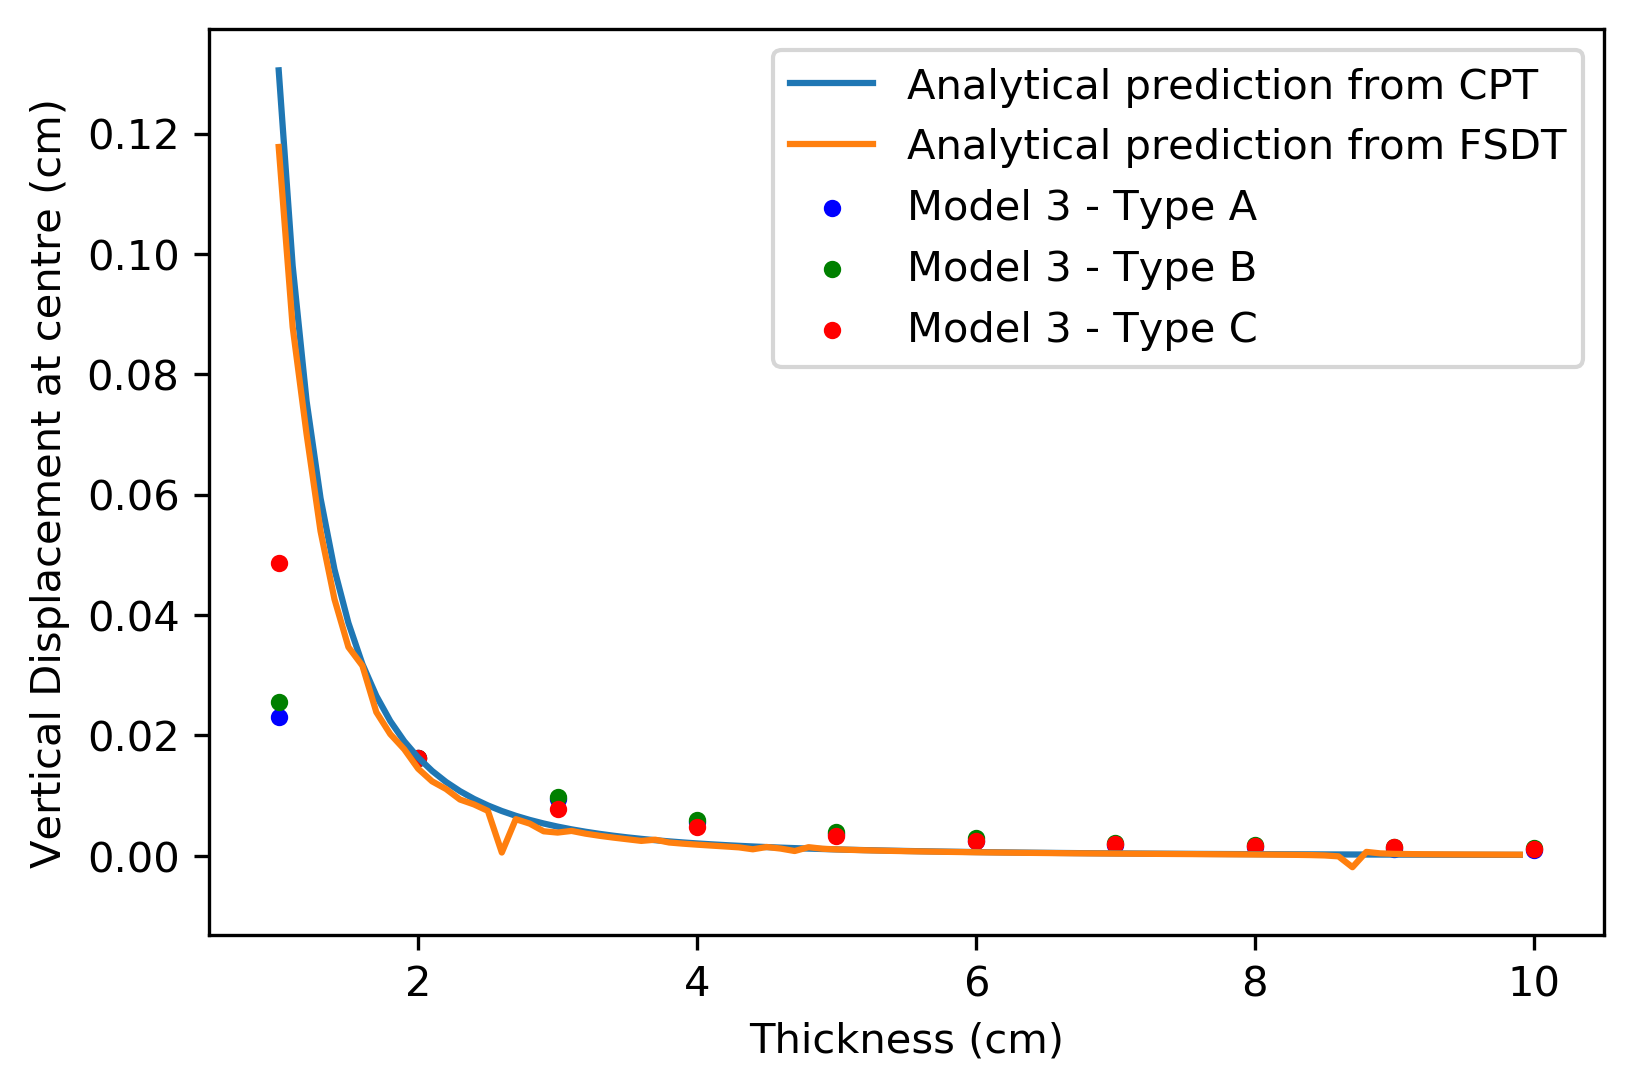
\includegraphics{Figures/M3_t_plt.png}
     \caption{Model 3 - Vertical Displacement with respect to Thickness for a Constant Vertical Load of 2 kN}
     \label{fig:M3_t_plt}
 \end{figure}
 
 \begin{figure}[!htbp]
     \centering
     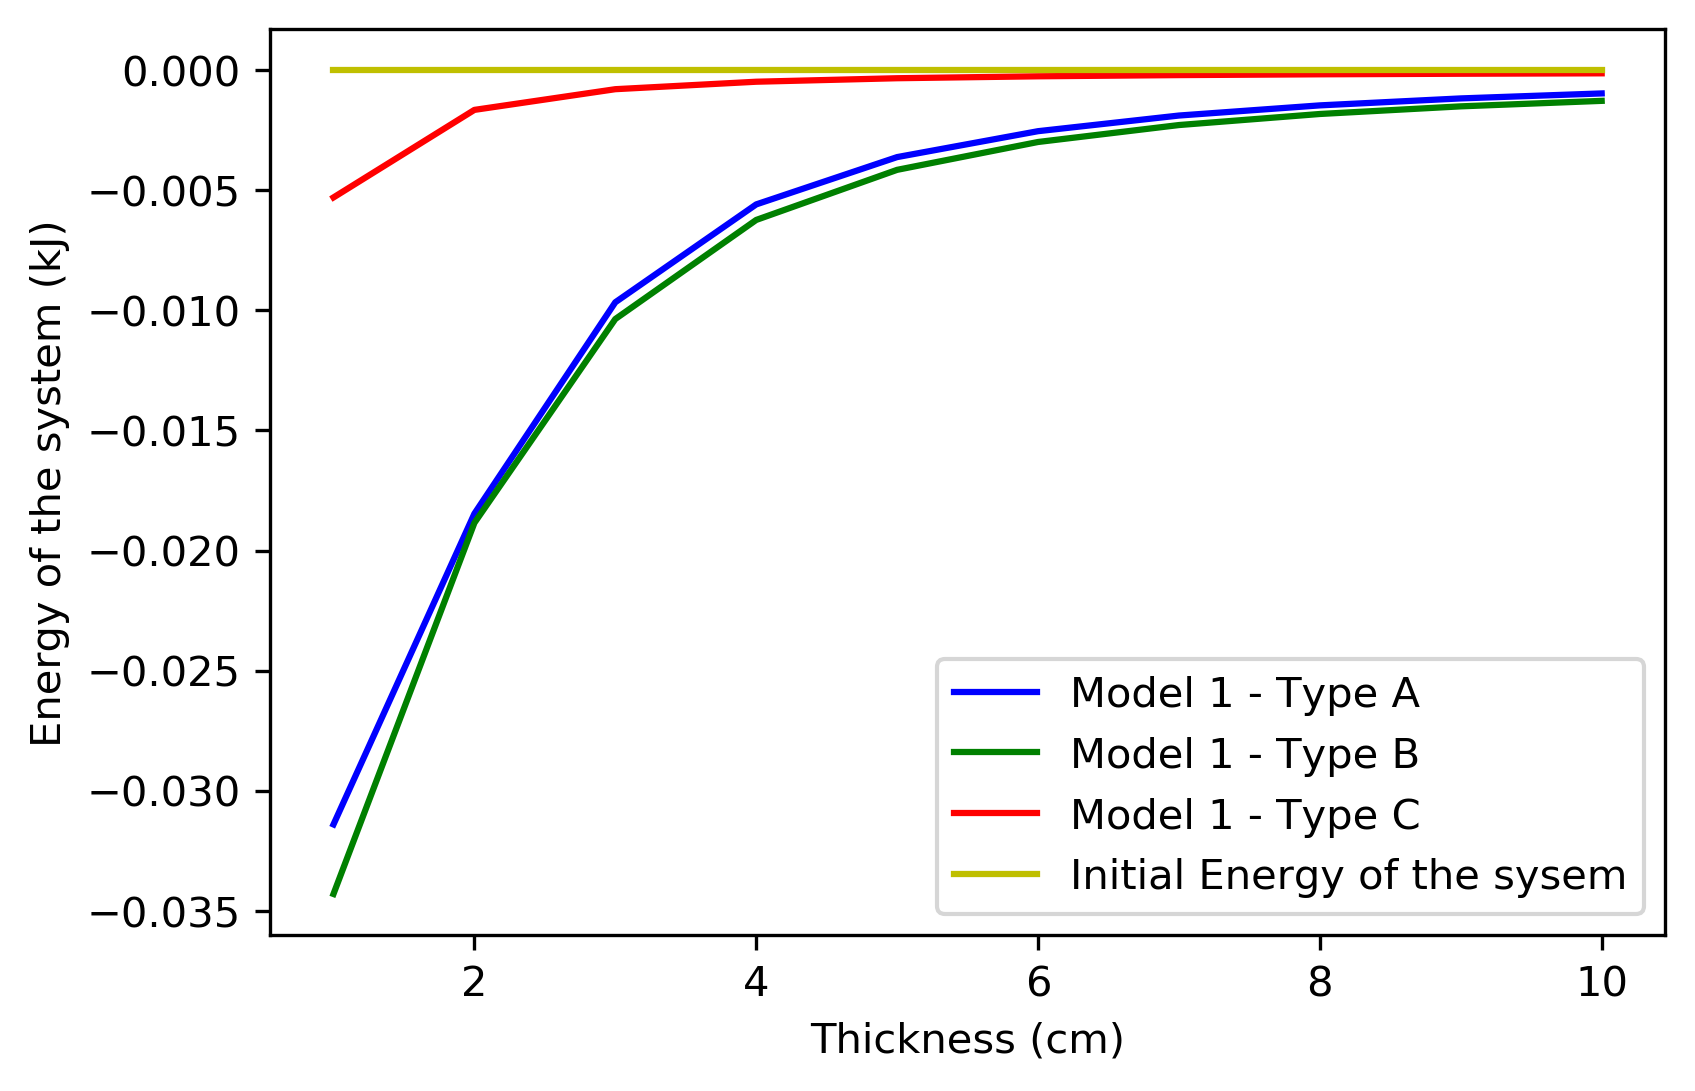
\includegraphics{Figures/M3_t_energy.png}
     \caption{Model 3 - Change in energy with respect to Thickness for a Constant Vertical Load of 2 kN}
     \label{fig:M3_t_energy}
 \end{figure}
 
 \section{Arbitrary Strain Fields}
 This section present the behavior of model under some strain for which qualitative shapes can be found in literature or by notions. Following this the deformed shapes under completely arbitrary strain fields are presented. The strain fields are translated into the model through the changes in natural lengths of the springs present in the model. Since Model 3 - Type C (1~m x 1~m x 0.02~m) performs best and predicts the results closest to the analytical solutions, it is used here to predict the deformed shapes.
 
 \subsection{Homogeneous Strain Field}
 All the horizontal springs of the model are modified such that the natural length of the springs are 10\% higher than their length in the undeformed state. This represents a strain field given by eq~\ref{eq:constant_xx_yy}
 
\begin{equation}
    \epsilon_{xx} = \epsilon_{yy} = Constant
    \label{eq:constant_xx_yy}
\end{equation}

All other strains are zero, however since the vertical springs do not have infinite stiffness, $\epsilon_{zz} \neq 0$. The qualitative deformed shape from the model is shown in the fig~\ref{fig:uniform_xxyy_xy} - fig~\ref{fig:uniform_xxyy_3d}. As expected, we can see a bulge at the centre when plate tries to expand in X- and Y- directions with all its edges simply supported.  The orange spring indicates the springs whose natural lengths have been changed.

\begin{figure}[!htbp]
\begin{minipage}{0.3\textwidth}
    \centering
    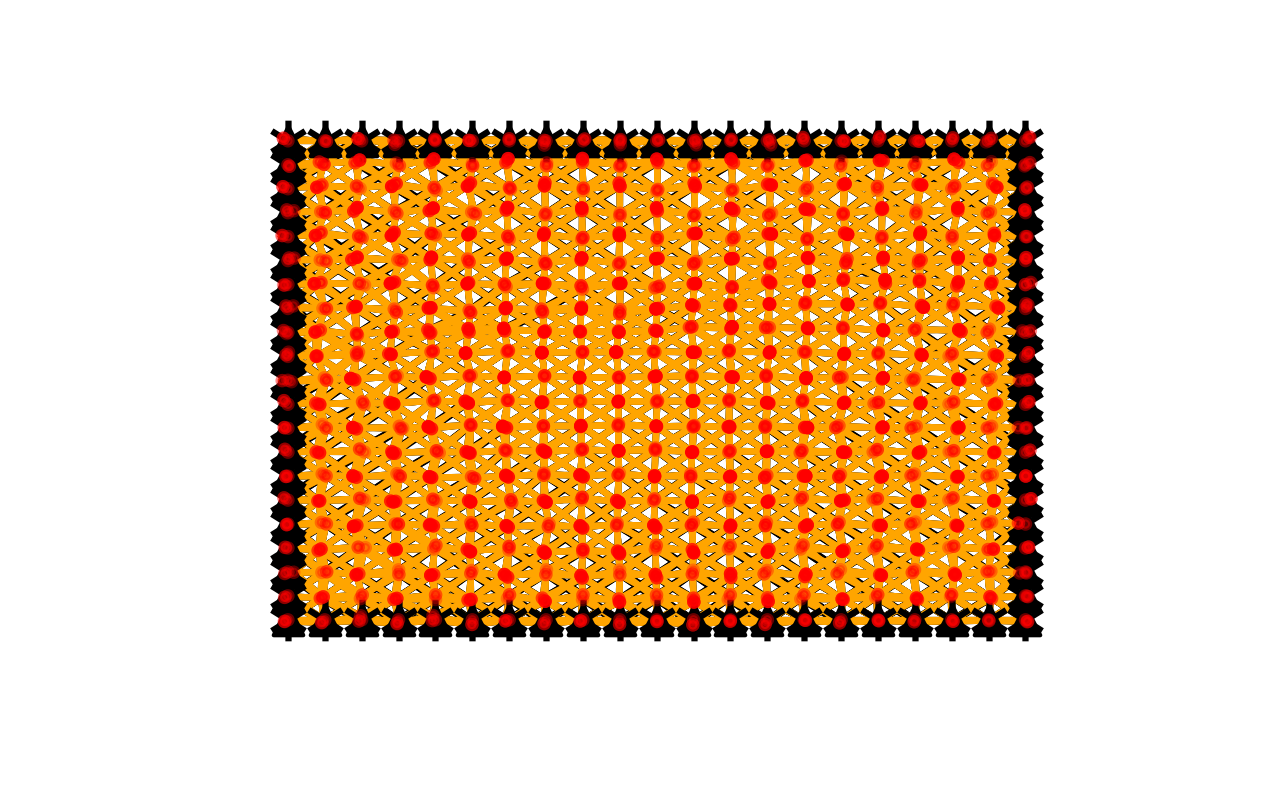
\includegraphics[width = 1\textwidth]{Figures/Uniform_XY_xxyy.png}
    \caption{Deformed shape - XY-view - uniform strain in X- and Y- direction}
    \label{fig:uniform_xxyy_xy}
\end{minipage}
\hspace{5mm}
\begin{minipage}{0.3\textwidth}
    \centering
    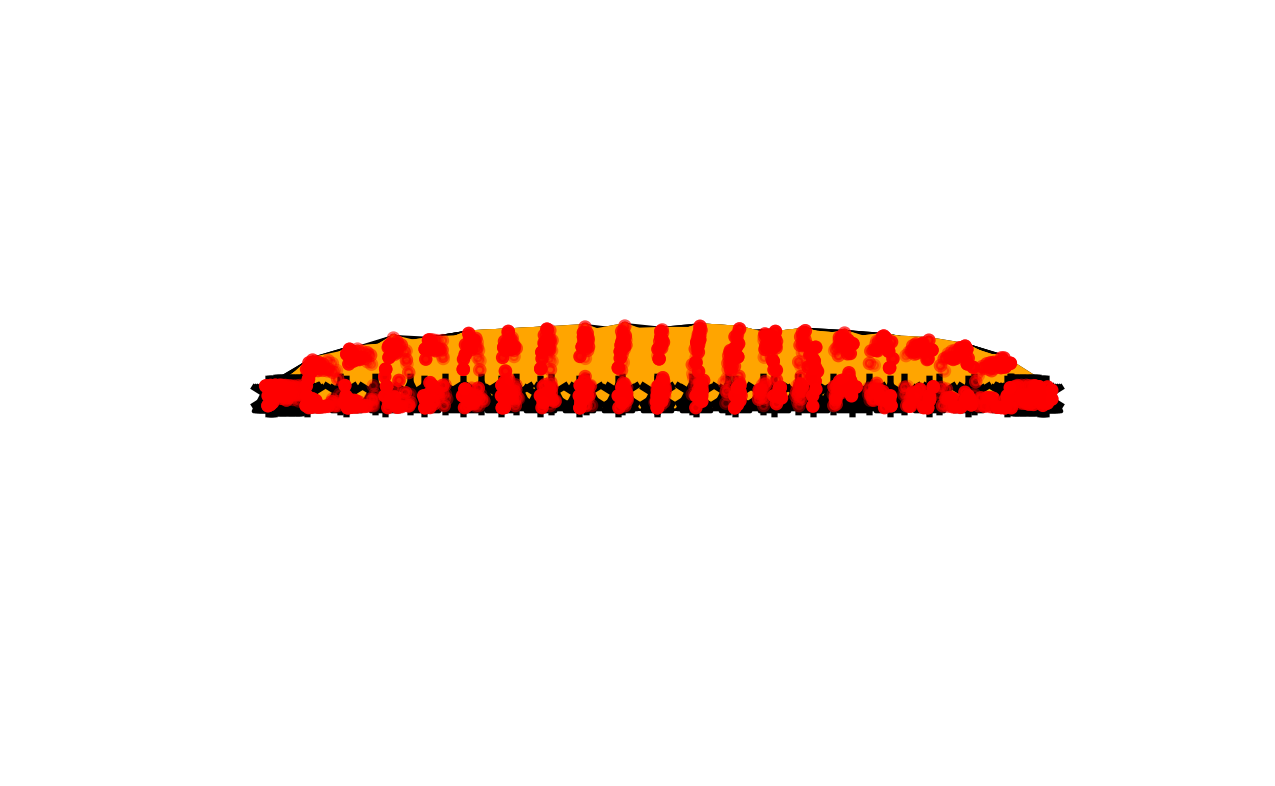
\includegraphics[width = 1\textwidth]{Figures/Uniform_YZ_xxyy.png}
    \caption{Deformed shape - YZ-view - uniform strain in X- and Y- direction}
    \label{fig:uniform_xxyy_yz}
\end{minipage}
\hspace{5mm}
\begin{minipage}{0.3\textwidth}
    \centering
    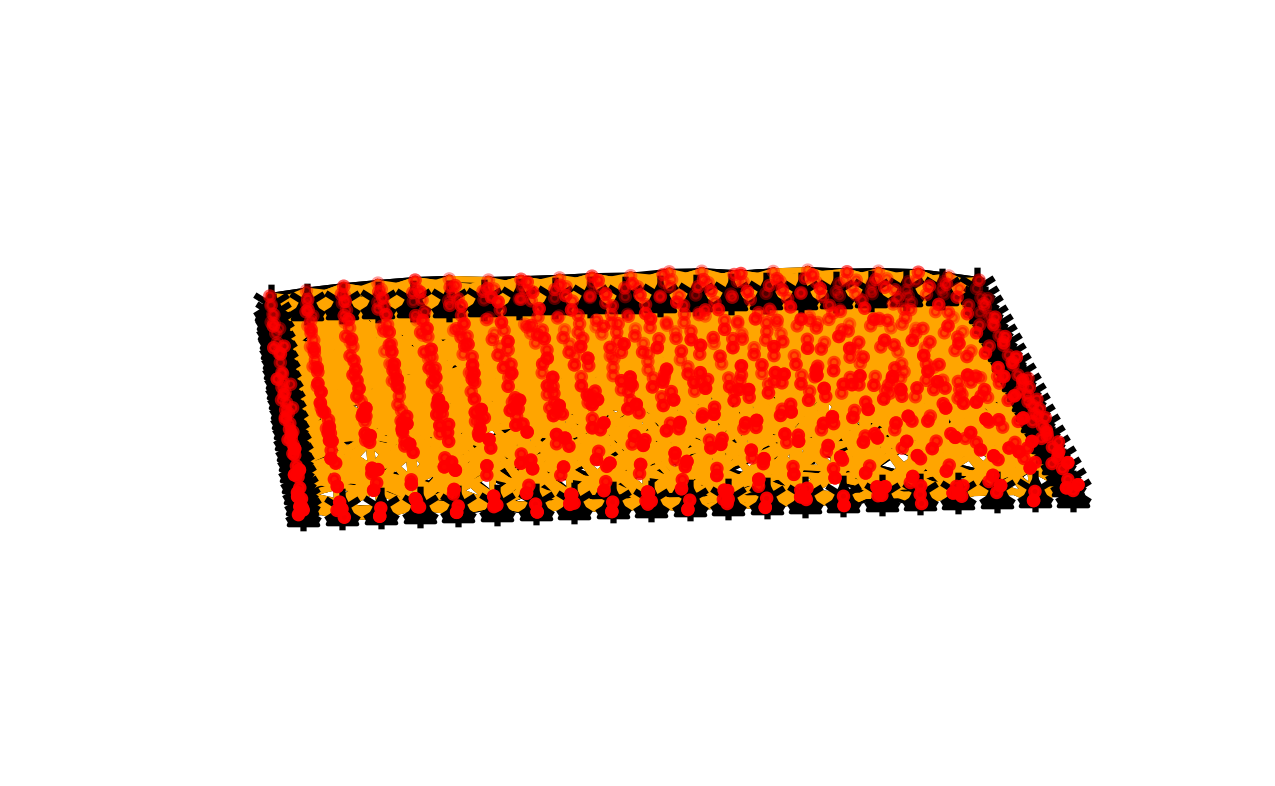
\includegraphics[width = 1\textwidth]{Figures/Uniform_3D_xxyy.png}
    \caption{Deformed shape - 3D-view - uniform strain in X- and Y- direction}
    \label{fig:uniform_xxyy_3d}
\end{minipage}
\end{figure}

Similar results were obtained for the case where:
\begin{equation}
    \epsilon_{zz} = Constant
\end{equation}
All other strain are zero. 

The deformed profile of the plate model is shown in the fig~\ref{fig:uniform_zz_xy} - fig~\ref{fig:uniform_zz_3d}. Comparing the two cases we can see that while the bulge in case where $\epsilon_{xx} = \epsilon_{yy} = Constant$, the bulge at the centre is distributed across the plate while for $\epsilon_{zz} = Constant$ case, the bulge is higher and is concentrated at the centre.

\begin{figure}[!htbp]
\begin{minipage}{0.3\textwidth}
    \centering
    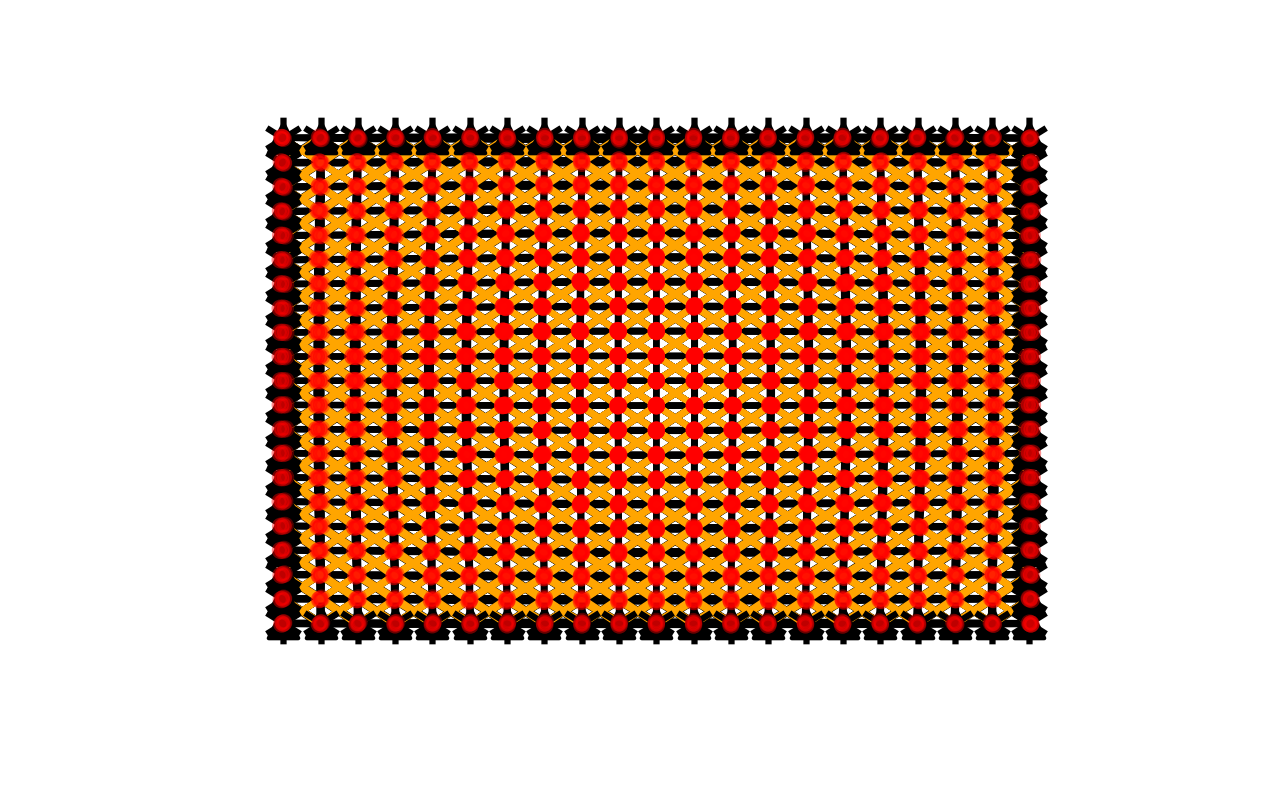
\includegraphics[width = 1\textwidth]{Figures/Uniform_XY_zz.png}
    \caption{Deformed shape - XY-view - uniform strain in Z- direction}
    \label{fig:uniform_zz_xy}
\end{minipage}
\hspace{5mm}
\begin{minipage}{0.3\textwidth}
    \centering
    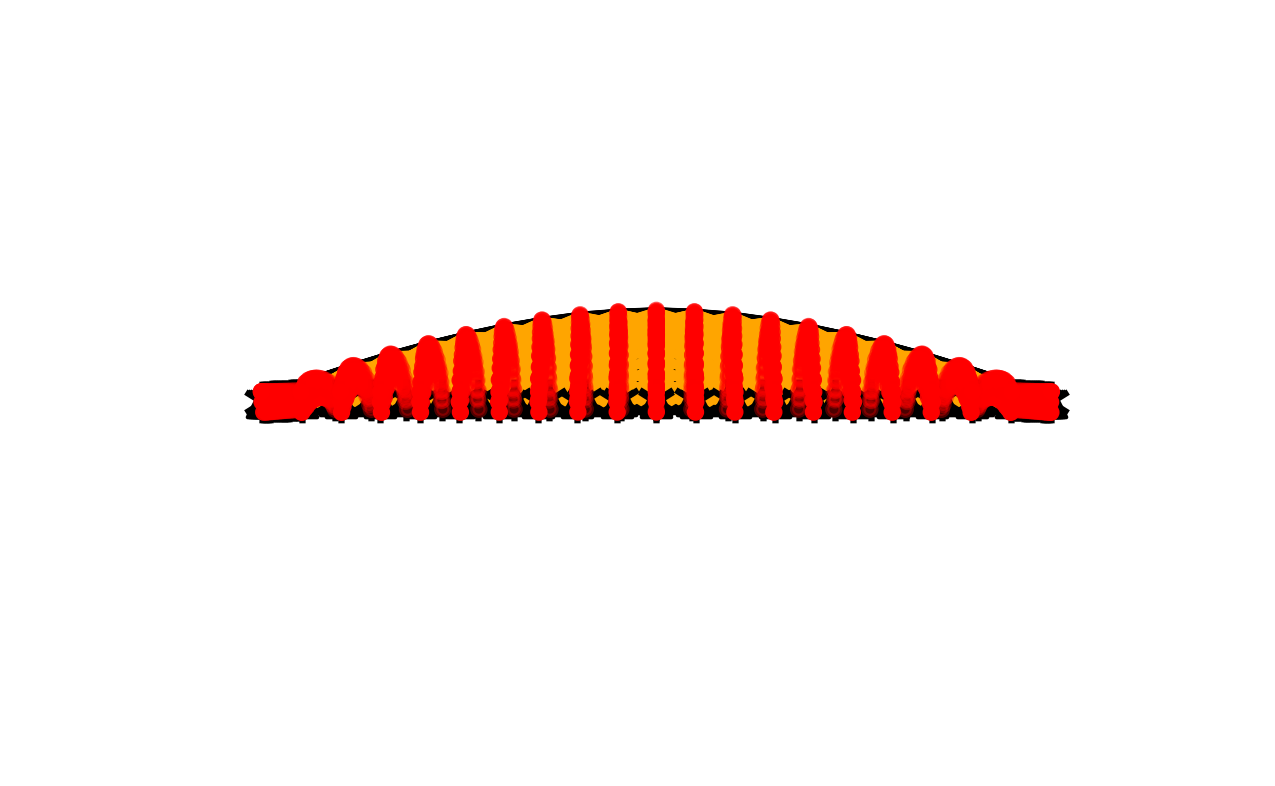
\includegraphics[width = 1\textwidth]{Figures/Uniform_YZ_zz.png}
    \caption{Deformed shape - YZ-view - uniform strain in Z- direction}
    \label{fig:uniform_zz_yz}
\end{minipage}
\hspace{5mm}
\begin{minipage}{0.3\textwidth}
    \centering
    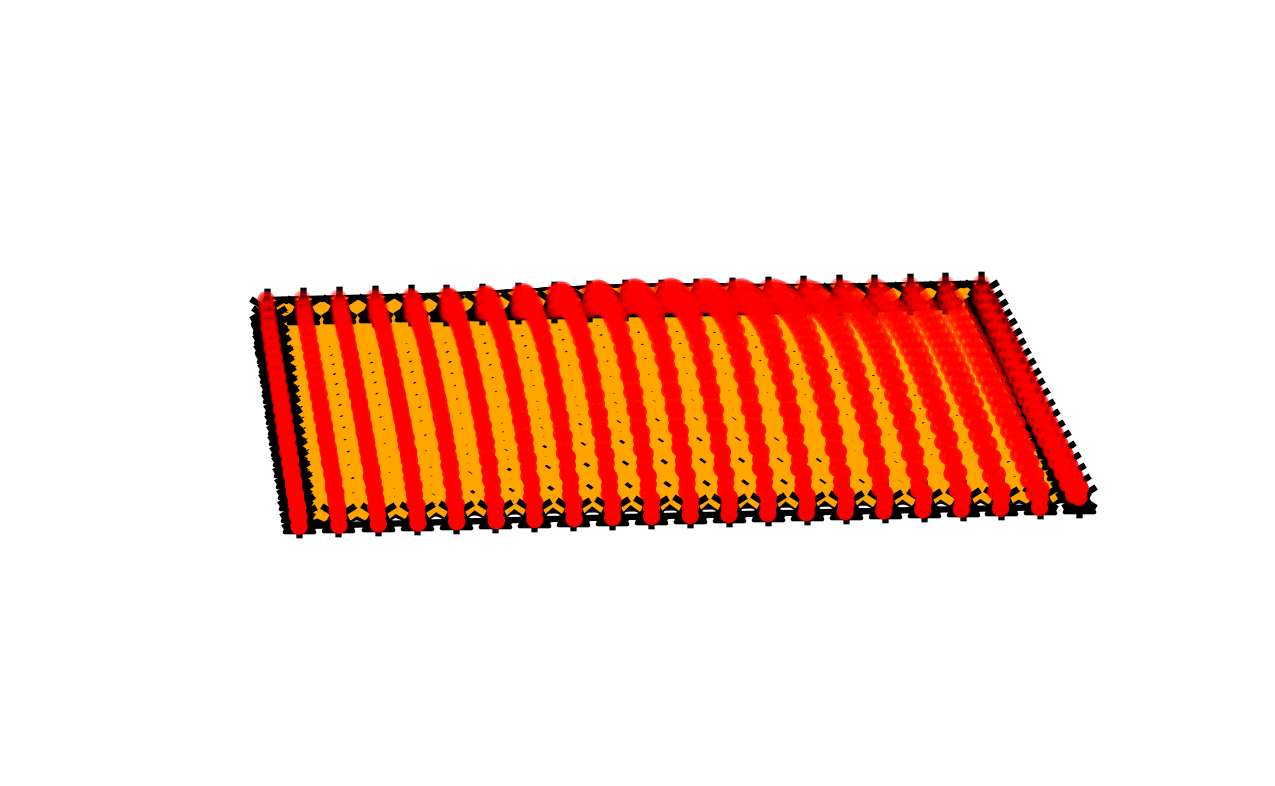
\includegraphics[width = 1\textwidth]{Figures/Uniform_3D_zz.png}
    \caption{Deformed shape - 3D-view - uniform strain in Z- direction}
    \label{fig:uniform_zz_3d}
\end{minipage}
\end{figure}

 \subsection{Temperature Gradient}
 Temperature gradient is model by selectively changing the natural length of springs in different layer. In our model, since there are three layers, the temperature gradient is simulated by increasing the natural length of the springs in top most layer and decreasing the natural length of the springs in bottom most layers while keeping the natural lengths of springs in middle layer unchanged. This represents the condition when the middle plane of plate is neutral and there are no normal strains in X- and Y- direction on the middle plane. Fig~\ref{fig:temp_grad_xy} - fig~\ref{fig:temp_grad_3d} show the deformed profile. As expected, plate has warped providing space to spring for elongation.
 
 \begin{figure}[!htbp]
\begin{minipage}{0.3\textwidth}
    \centering
    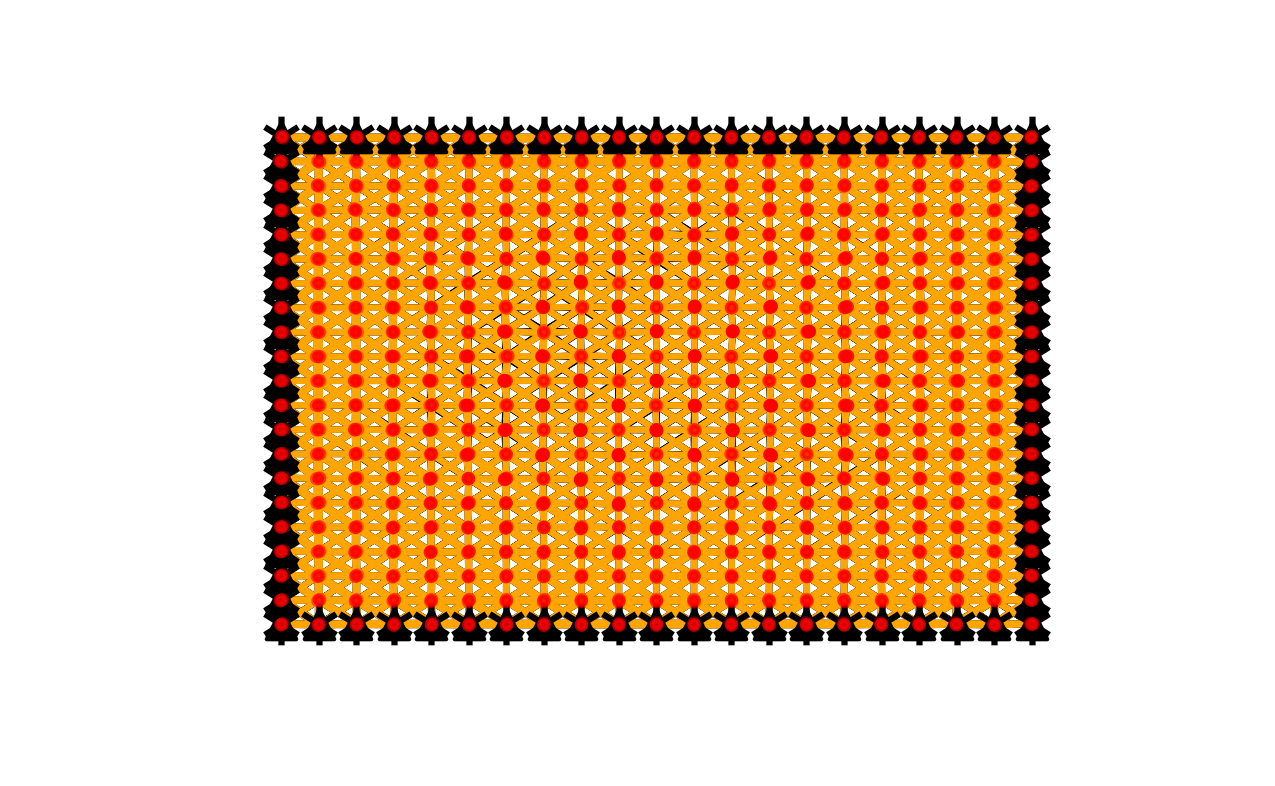
\includegraphics[width = 1\textwidth]{Figures/temp_grad_XY.png}
    \caption{Deformed shape - XY-view - Temperature Gradient}
    \label{fig:temp_grad_xy}
\end{minipage}
\hspace{5mm}
\begin{minipage}{0.3\textwidth}
    \centering
    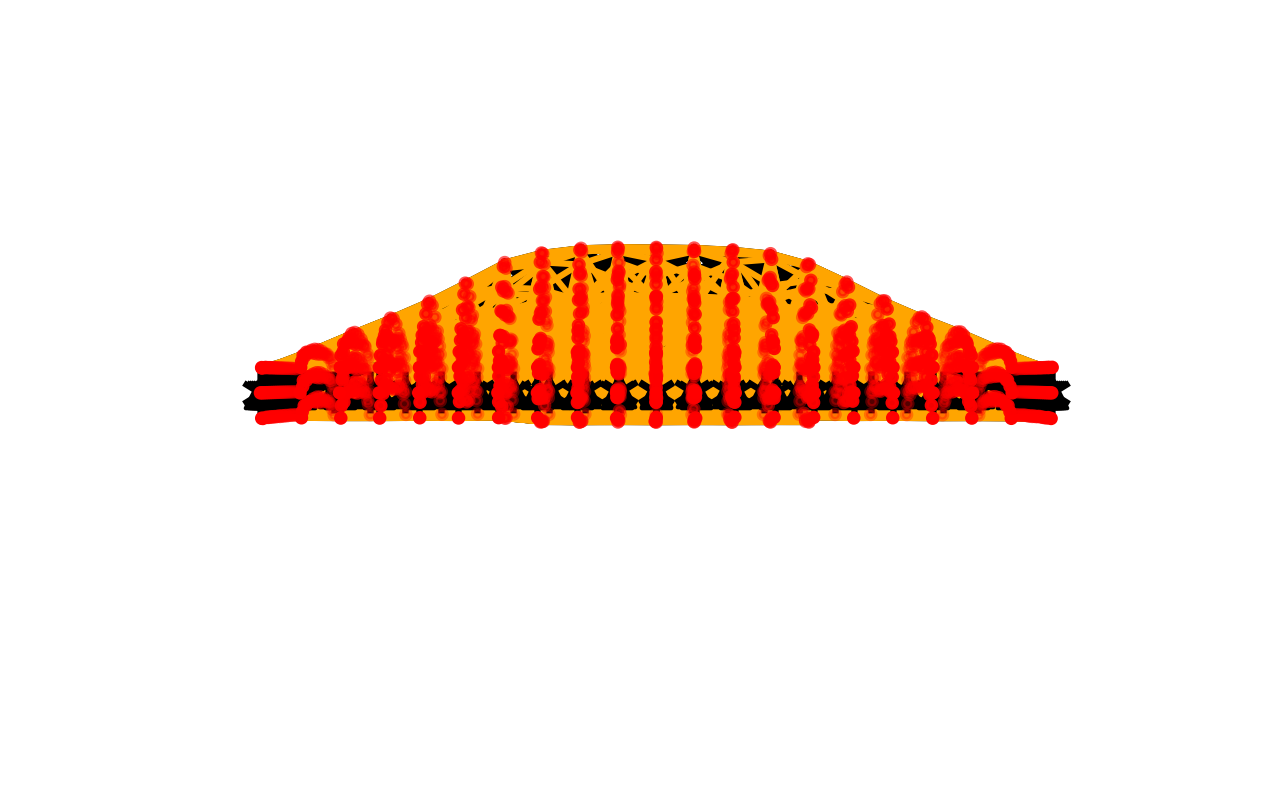
\includegraphics[width = 1\textwidth]{Figures/temp_grad_YZ.png}
    \caption{Deformed shape - YZ-view - Temperature Gradient}
    \label{fig:temp_grad_yz}
\end{minipage}
\hspace{5mm}
\begin{minipage}{0.3\textwidth}
    \centering
    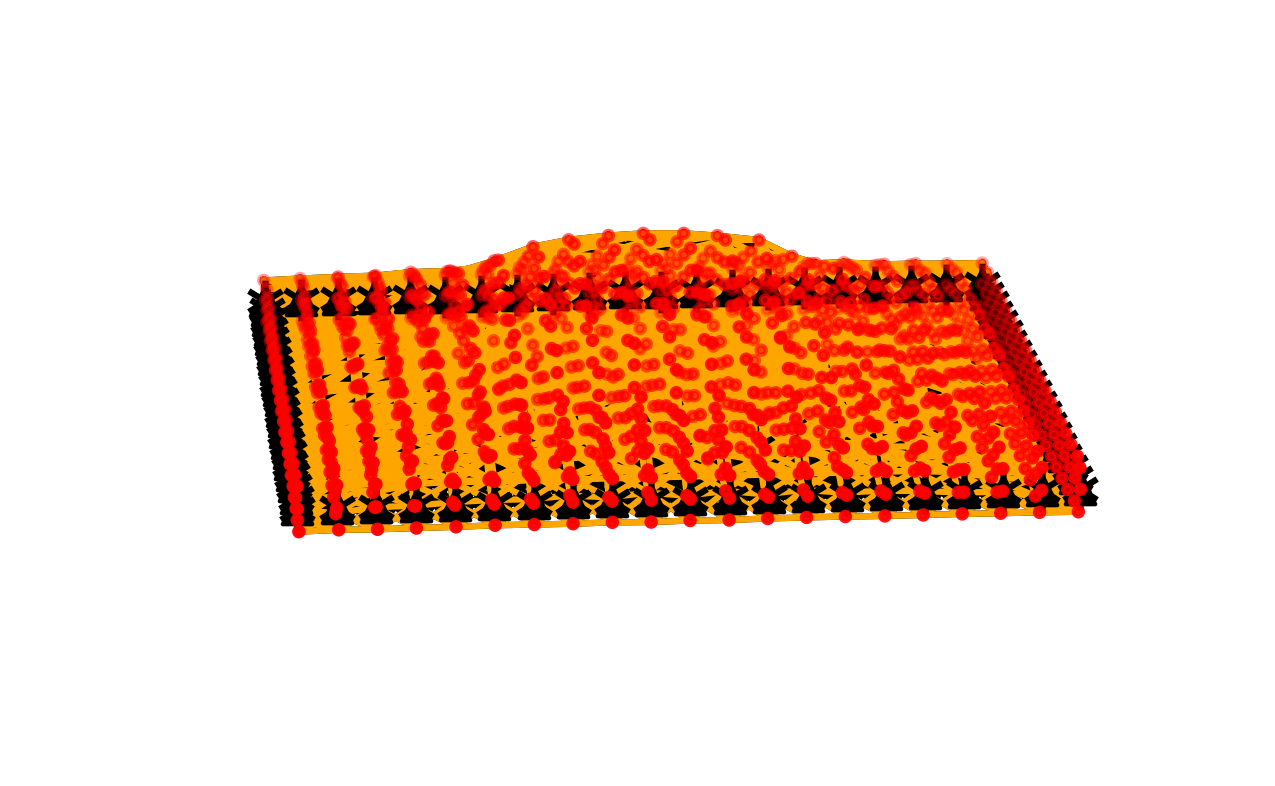
\includegraphics[width = 1\textwidth]{Figures/temp_grad_3D.png}
    \caption{Deformed shape - 3D-view - Temperature Gradient}
    \label{fig:temp_grad_3d}
\end{minipage}
\end{figure}

\subsection{Radial Strain Field}
Deformed lattices shown in the fig~\ref{fig:radial_strain_xy} - fig~\ref{fig:radial_strain_3d} presents the stain field given by:

\begin{equation}
    \epsilon_{rr} = Constant \quad \textrm{for} \, r\leq 0.25
\end{equation}
Origin of the Cylindrical co-ordinate system located at the centre of the plate and all other strains being zero.

As expected we can find the deformed shape expanding at the centre to provide space for springs to grow. The springs in Orange represents the springs with altered natural length.

\begin{figure}[!htbp]
\begin{minipage}{0.3\textwidth}
    \centering
    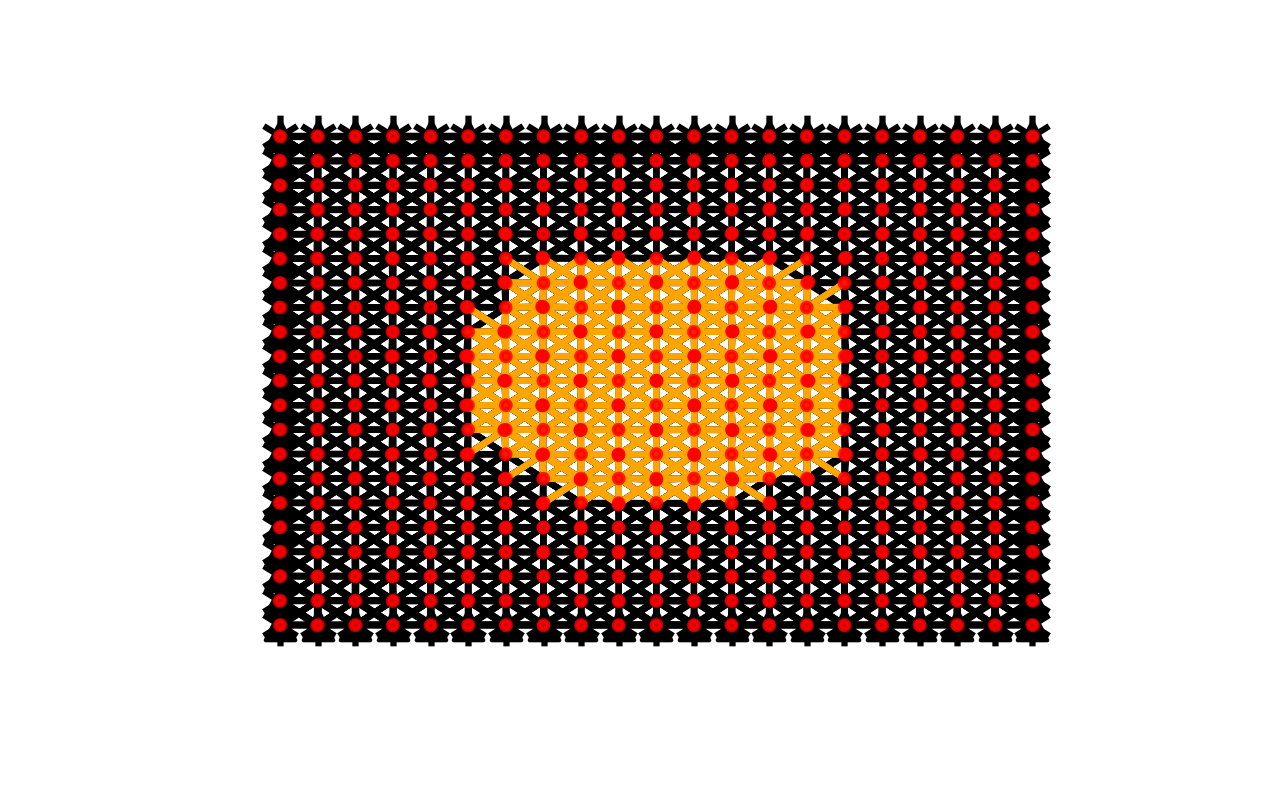
\includegraphics[width = 1\textwidth]{Figures/circ_XY.png}
    \caption{Deformed shape - XY-view - Radial Strain Field}
    \label{fig:radial_strain_xy}
\end{minipage}
\hspace{5mm}
\begin{minipage}{0.3\textwidth}
    \centering
    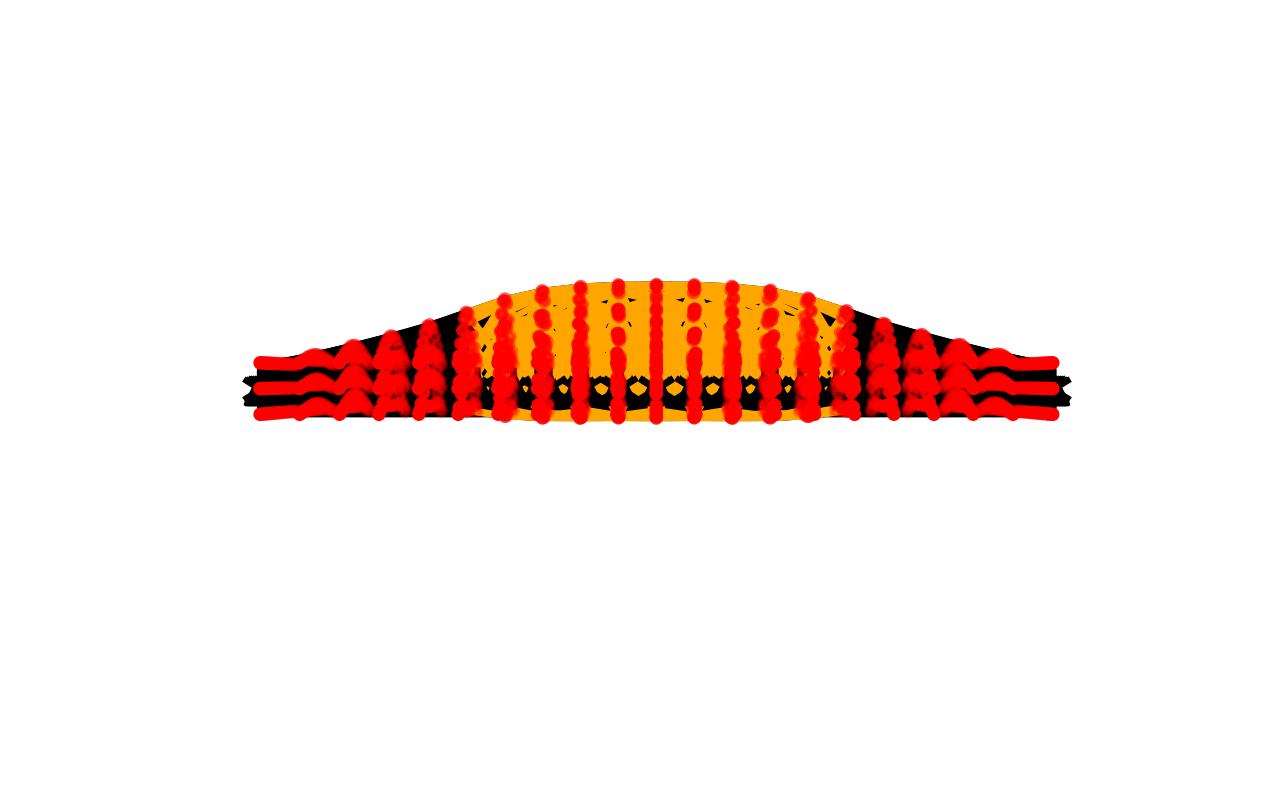
\includegraphics[width = 1\textwidth]{Figures/circ_YZ.png}
    \caption{Deformed shape - YZ-view - Radial Strain Field}
    \label{fig:radial_strain_yz}
\end{minipage}
\hspace{5mm}
\begin{minipage}{0.3\textwidth}
    \centering
    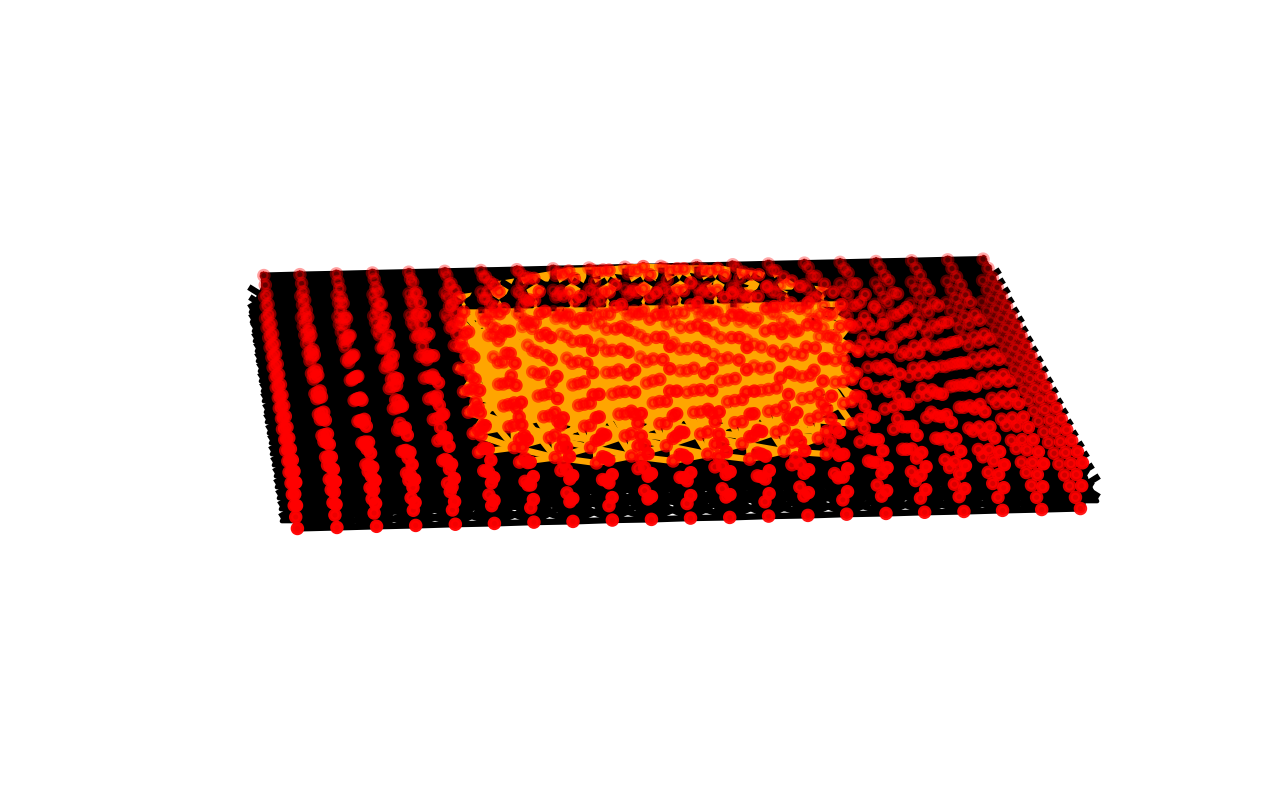
\includegraphics[width = 1\textwidth]{Figures/circ_3D.png}
    \caption{Deformed shape - 3D-view - Radial Strain Field}
    \label{fig:radial_strain_3d}
\end{minipage}
\end{figure}

\newpage
\subsection{Random Strain Fields}
This section provides deformed shapes of the model under completely random strain fields obtained by randomly selecting any number of springs and modifying their natural length.

\subsubsection{Case 1}
5\% of the total springs have altered natural length.
\begin{figure}[!htbp]
\begin{minipage}{0.3\textwidth}
    \centering
    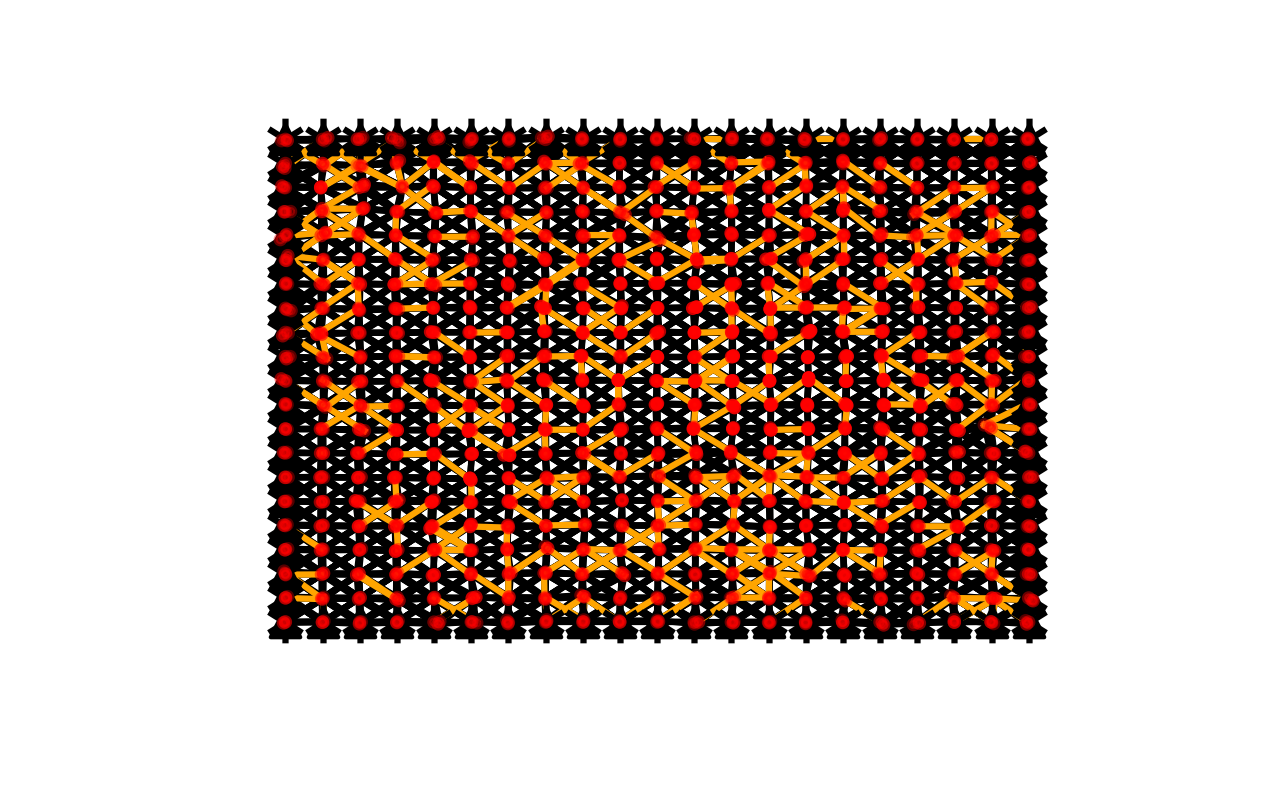
\includegraphics[width = 1\textwidth]{Figures/rand_5_XY.png}
    \caption{Deformed shape - XY-view - 5\% random springs}
    \label{fig:rand_5_xy}
\end{minipage}
\hspace{5mm}
\begin{minipage}{0.3\textwidth}
    \centering
    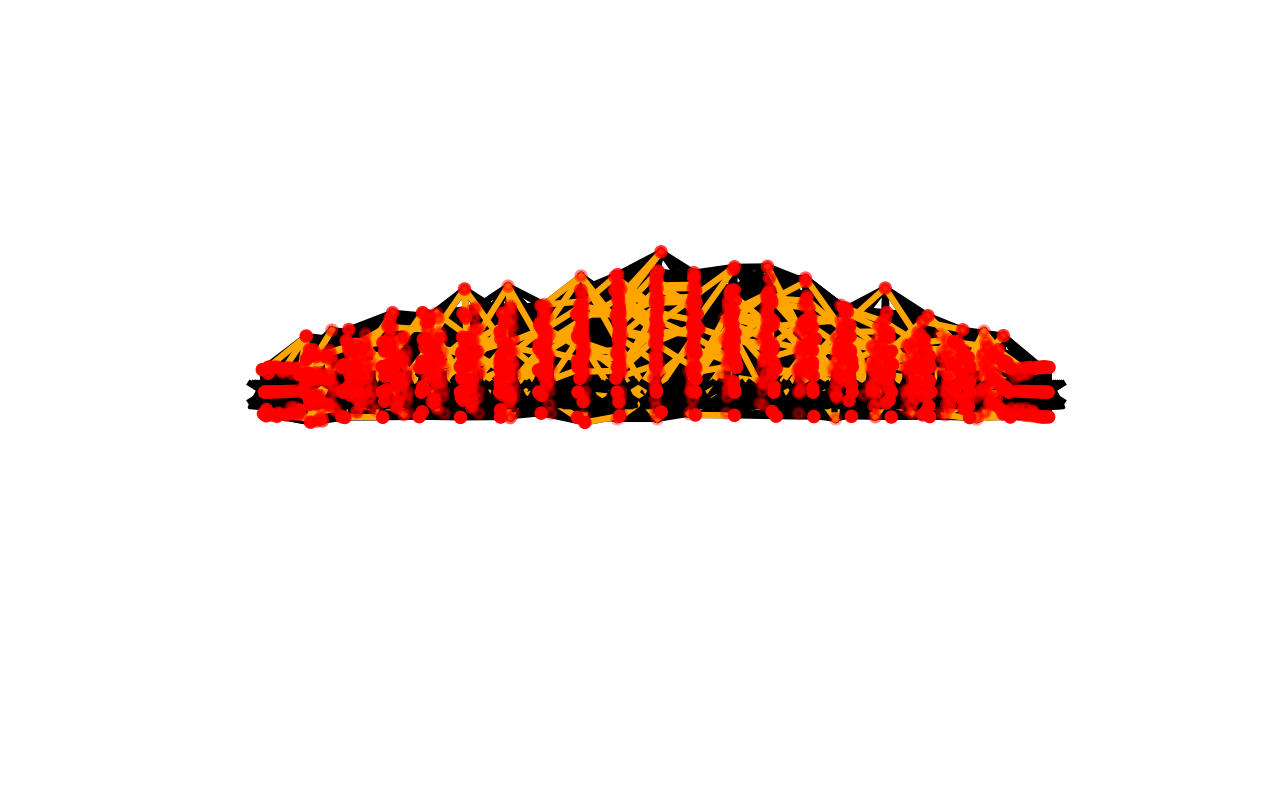
\includegraphics[width = 1\textwidth]{Figures/rand_5_YZ.png}
    \caption{Deformed shape - YZ-view - 5\% random springs}
    \label{fig:rand_5_yz}
\end{minipage}
\hspace{5mm}
\begin{minipage}{0.3\textwidth}
    \centering
    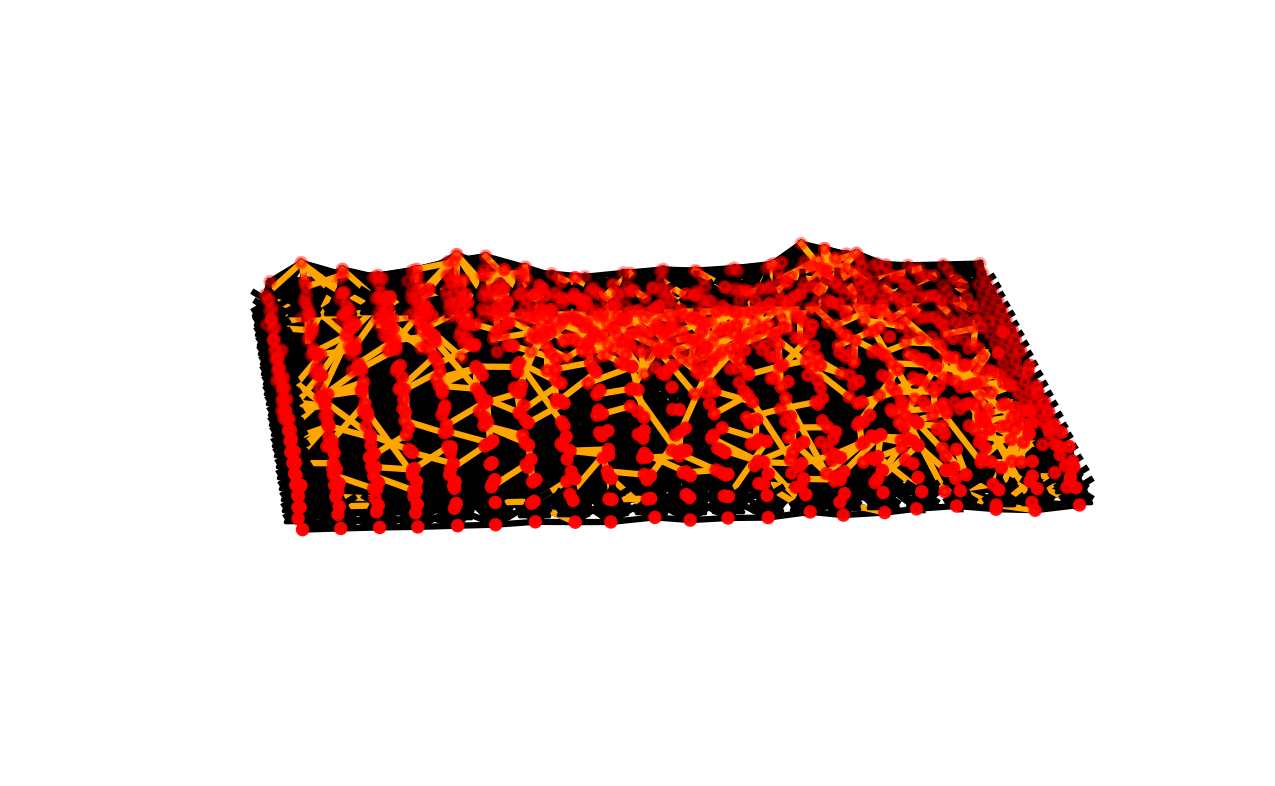
\includegraphics[width = 1\textwidth]{Figures/rand_5_3D.png}
    \caption{Deformed shape - 3D-view - 5\% random springs}
    \label{fig:rand_5_3d}
\end{minipage}
\end{figure}

\subsubsection{Case 2}
10\% of the total springs have altered natural length.
\begin{figure}[!htbp]
\begin{minipage}{0.3\textwidth}
    \centering
    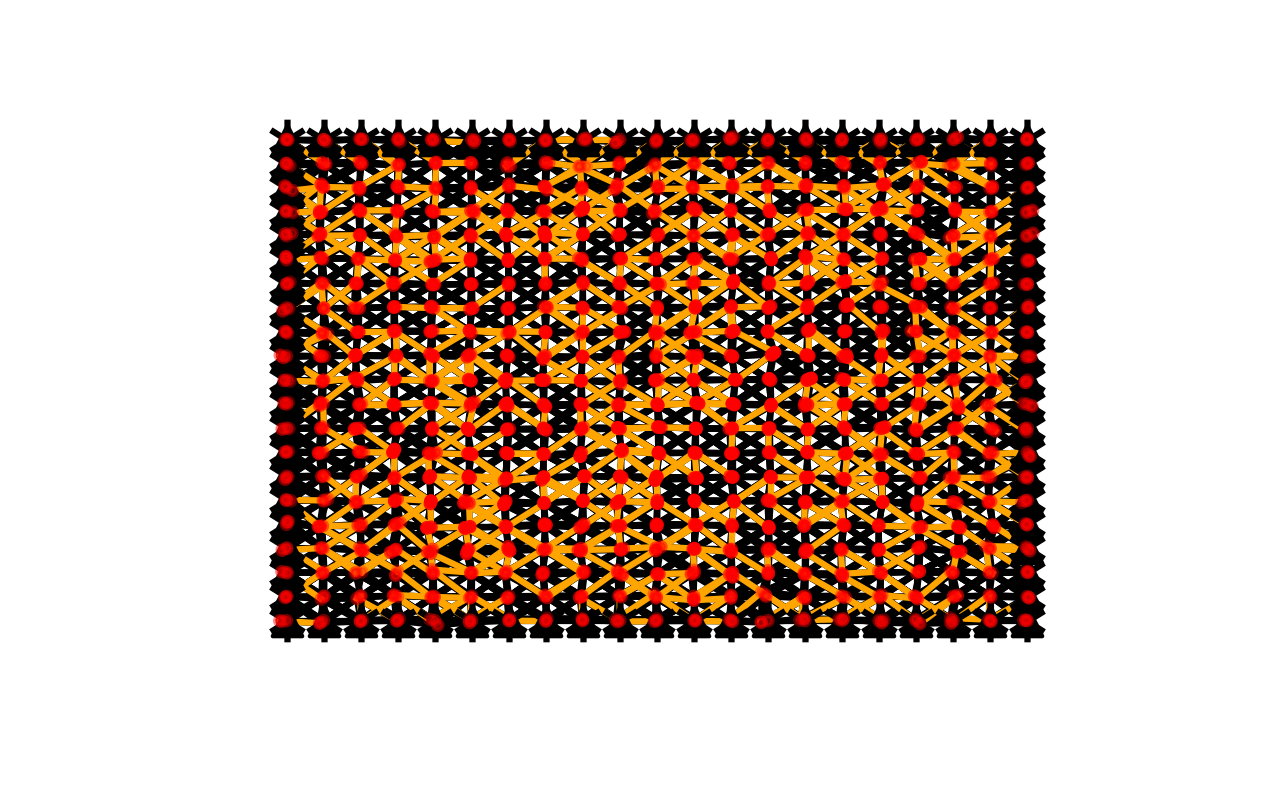
\includegraphics[width = 1\textwidth]{Figures/rand_10_XY.png}
    \caption{Deformed shape - XY-view - 10\% random springs}
    \label{fig:rand_10_xy}
\end{minipage}
\hspace{5mm}
\begin{minipage}{0.3\textwidth}
    \centering
    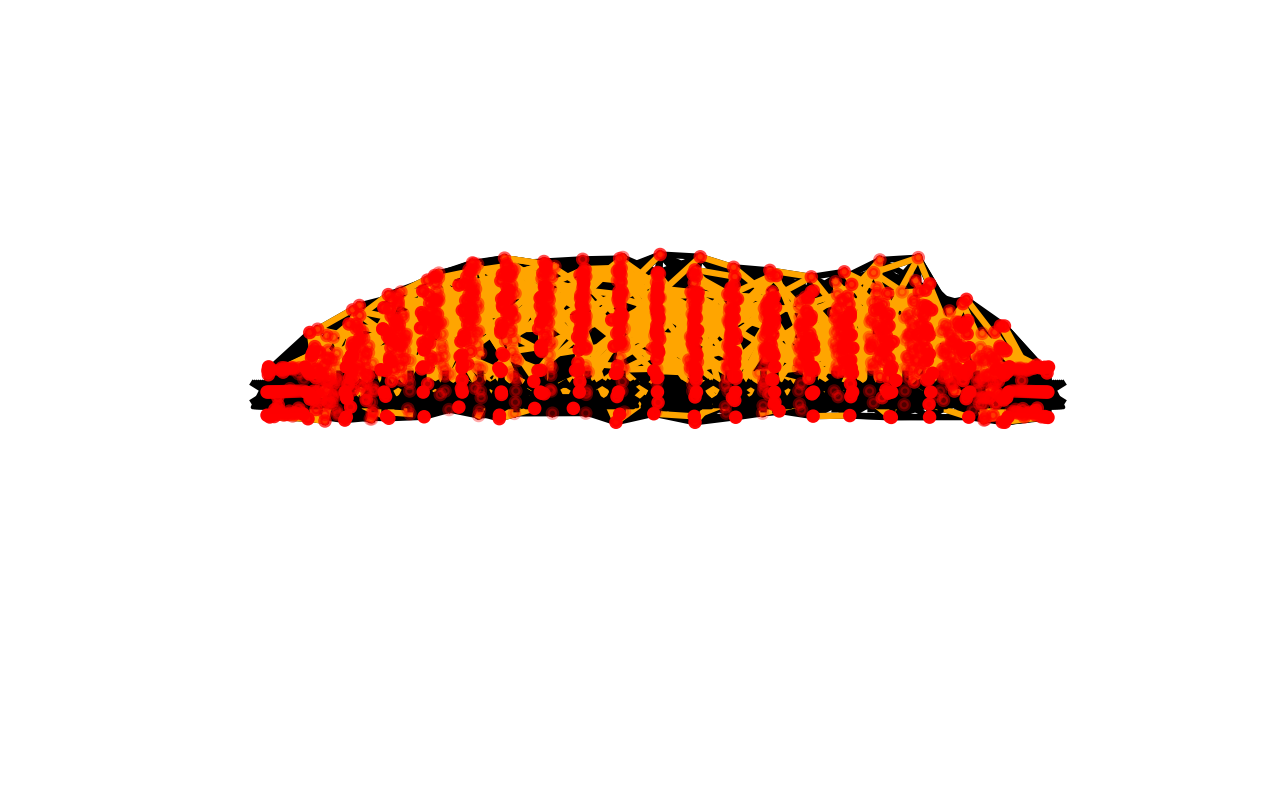
\includegraphics[width = 1\textwidth]{Figures/rand_10_YZ.png}
    \caption{Deformed shape - YZ-view - 10\% random springs}
    \label{fig:rand_10_yz}
\end{minipage}
\hspace{5mm}
\begin{minipage}{0.3\textwidth}
    \centering
    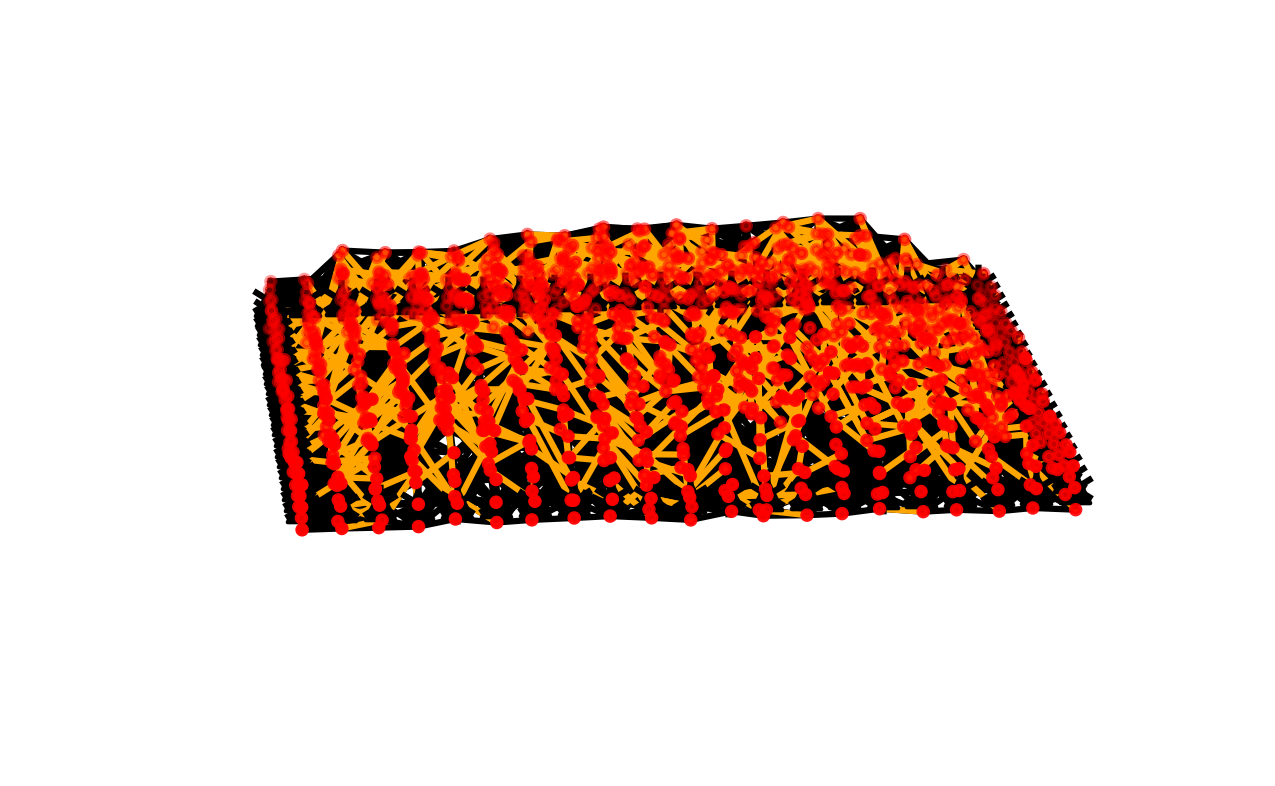
\includegraphics[width = 1\textwidth]{Figures/rand_10_3D.png}
    \caption{Deformed shape - 3D-view - 10\% random springs}
    \label{fig:rand_10_3d}
\end{minipage}
\end{figure}

\subsubsection{Case 3}
50\% of the total springs have altered natural length.
\begin{figure}[!htbp]
\begin{minipage}{0.3\textwidth}
    \centering
    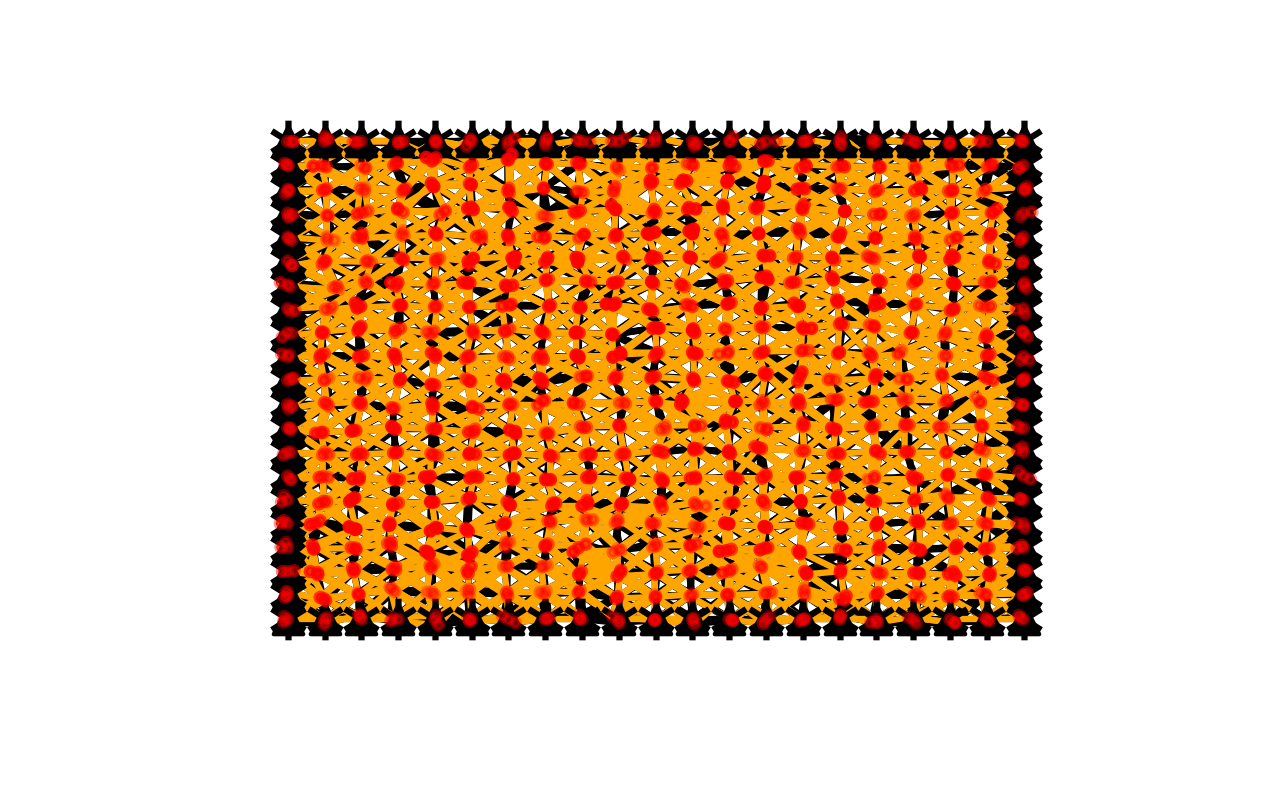
\includegraphics[width = 1\textwidth]{Figures/rand_50_XY.png}
    \caption{Deformed shape - XY-view - 50\% random springs}
    \label{fig:rand_50_xy}
\end{minipage}
\hspace{5mm}
\begin{minipage}{0.3\textwidth}
    \centering
    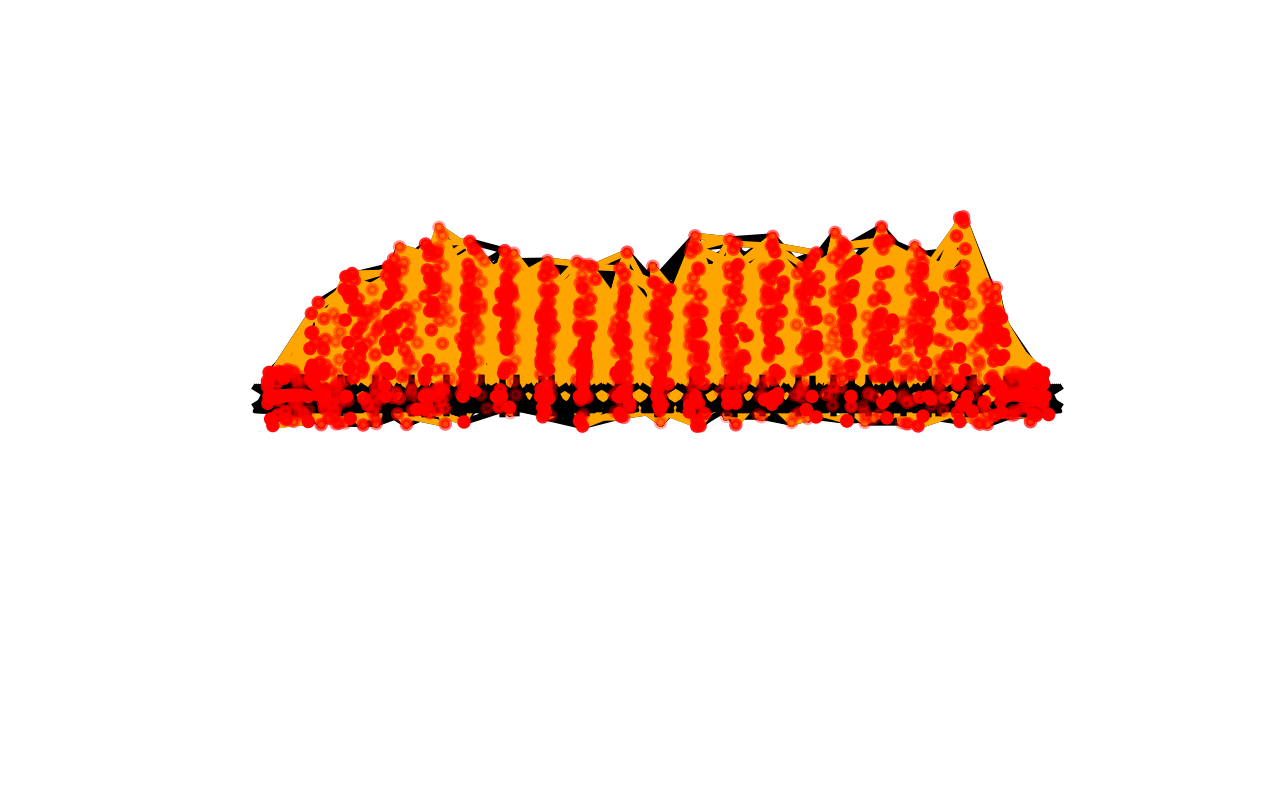
\includegraphics[width = 1\textwidth]{Figures/rand_50_YZ.png}
    \caption{Deformed shape - YZ-view - 50\% random springs}
    \label{fig:rand_50_yz}
\end{minipage}
\hspace{5mm}
\begin{minipage}{0.3\textwidth}
    \centering
    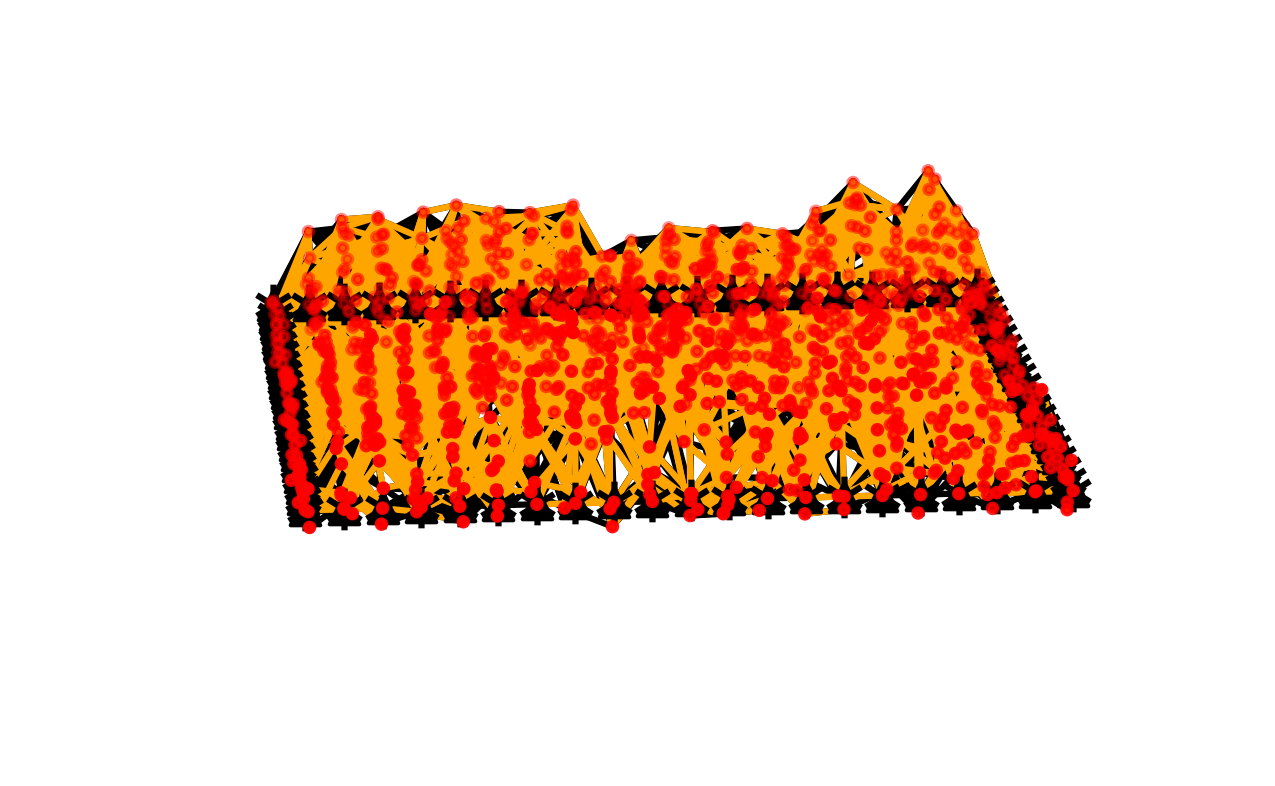
\includegraphics[width = 1\textwidth]{Figures/rand_50_3D.png}
    \caption{Deformed shape - 3D-view - 50\% random springs}
    \label{fig:rand_50_3d}
\end{minipage}
\end{figure}

\newpage
\section{Conclusion}
From the points presented above, we can see that:
\begin{enumerate}
    \item Model 3 predictions match well with the analytical result obtained from Classical Plate theory and First-order Shear Deformation theory. Model 1 and Model 2 appear to be insensitive to thickness variations. This behavior is also reflected in the plots of Energy Change vs Thickness.
    \item The model predicts deformed shape which are qualitatively in good agreement with the expected shapes. Models predictions of deformed shape are also shown for cases when any random 5\%, 10\%, and 50\% springs have their natural length altered, indicating that any arbitrary strain field can be simulated provided we can translate the strain field to a pattern in which springs natural length is to be altered.
\end{enumerate}

\section{Limitations of Model and Suggested Improvements}
The limitation and suggested improvements for the model based on the above study are as follows:
\begin{enumerate}
    \item As it can be seen from the outputs of the model under section titled 'Random Strain Fields', the deformed shapes have kinks are which are not usually possible in plates. This is happening partly due the fact that spring ball joints have no rotational stiffness. Inability of the model to provide extremely high stiffness in the Z-direction also contributes to the problem. As discussed already in Section~\ref{sec:Limitations}, the problem can be overcome by providing a regularization term in the expression of design function for the minimization problem.
    \item Though some simple strain fields can be intuitively translated in pattern in which natural length of the springs in the model is to be altered and hence can get reflected in model. A routine needs to be developed which will be able to translate any given strain field to equivalent pattern of spring length changes. Alternatively, the position of the nodes can be changed in accordance with the strain field instead of natural length of springs.
    \item The violation of the assumption $\epsilon_{zz} = 0$ has lead to several kind of deviations from expected behavior and it might be helpful to model this behavior as constraint rather than using vertical springs with very high stiffness, since using springs of very high stiffness compared to other leads to numerical instability in the model. The increased computation time and effort can be lowered by providing analytical Hessian matrix. Also, these constraint might lead to better result even with lower number of nodes and springs, further reducing computation efforts by reducing number of design variables.
\end{enumerate}